\documentclass[a4paper,11pt]{article}
\usepackage{jheppub}
\usepackage{url}
\RequirePackage{color,graphicx}
\usepackage{mathtools}
\usepackage{amsfonts}
\usepackage{amsthm}
\begingroup
    \makeatletter
    \@for\theoremstyle:=definition,remark,plain\do{%
        \expandafter\g@addto@macro\csname th@\theoremstyle\endcsname{%
            \addtolength\thm@preskip\parskip
            }%
        }
\endgroup
\usepackage{parskip}
\usepackage{pgfplots}
\pgfplotsset{compat=1.14}
\usepackage{braket}
\usepackage{tensor}

\theoremstyle{definition}
\newtheorem*{defn}{Definition}
\newtheorem*{prop}{Proposition}
\newtheorem*{ex}{Example}
\newtheorem*{exs}{Examples}
\newtheorem*{thm}{Theorem}
\newtheorem*{lem}{Lemma}
\newtheorem*{cor}{Corollary}
\newtheorem*{rmks}{Remarks}

\DeclareMathOperator{\Int}{Int}
\DeclareMathOperator{\im}{im}

\newcommand\numberthis{\addtocounter{equation}{1}\tag{\theequation}}

\tikzstyle{circ} = [circle, minimum width=1.5mm, inner sep=0pt,draw,fill]

\numberwithin{equation}{section}

\makeatletter
\def\@fpheader{
    %
}
\makeatother
\title{Metric and Topological Spaces}

\author{Mathematical Tripos Part 1B}
\affiliation{University of Cambridge}

\begin{document}
\maketitle
\flushbottom
\clearpage

\hrulefill

\textbf{Metrics.}
Definition and examples. Limits and continuity. Open sets and neighbourhoods.\\
Characterizing limits and continuity using neighbourhoods and open sets.

\textbf{Topology.}
Definition of a topology. Metric topologies. Further examples. Neighbourhoods, closed sets, convergence and continuity. Hausdorff spaces. Homeomorphisms. Topological and non-topological properties. Completeness. Subspace, quotient and product topologies.

\textbf{Connectedness.}
Definition using open sets and integer-valued functions. Examples, including intervals. Components. The continuous image of a connected space is connected. Path-connectedness. Path-connected spaces are connected but not conversely. Connected open sets in Euclidean space are path-connected.

\textbf{Compactness.}
Definition using open covers. Examples: finite sets and $[0, 1]$. Closed subsets of compact spaces are compact. Compact subsets of a Hausdorff space must be closed. The compact subsets of the real line. Continuous images of compact sets are compact. Quotient spaces. Continuous real-valued functions on a compact space are bounded and attain their bounds. The product of two compact spaces is compact. The compact subsets of Euclidean space. Sequential compactness.

\hrulefill
\clearpage

\section{Metric spaces}

\begin{defn}[Metric space]
A \emph{metric space} is a pair $(X, d_X)$ where $X$ is a set and $d_X$ is a function $d_X: X\times X\rightarrow\mathbb{R}$ s.t. for all $x,y,z$, 
\begin{enumerate}
    \item $d_X(x,y)\geq0$ (non-negativity)
    \item $d_X(x,y)=0$ iff $x=y$ (identity of indiscernibles)
    \item $d_X(x,y)=d_X(y,x)$ (symmetry)
    \item $d_X(x,y)\leq d_X(x,y)+d_X(y,z)$ (triangle inequality)
\end{enumerate}
\end{defn}

\begin{ex}[Usual Euclidean metric]
Let $X=\mathbb{R}^n$. Then for two vectors $\mathbf{v}, \mathbf{w}$,
\begin{equation}
    d(\mathbf{v},\mathbf{w}) = |\mathbf{v} - \mathbf{w}|=\sqrt{\sum_{i=1}^n (v_i-w_i)^2}
\end{equation}
is the usual notion of distance on an $\mathbb{R}^n$ vector space. It is not difficult to show that this indeed satisfies the conditions of a metric (the last condition comes from the Cauchy-Schwartz inequality).
\end{ex}

\begin{defn}[Metric subspace]
Let $(X,d_X)$ be a metric space, and $Y\subseteq X$. Then $(Y,d_Y)$ is a metric space and \emph{subspace} of $X$, where $d_Y(a,b)=d_X(a,b)$.
\end{defn}

This allows us to generate another metric space by picking out a subset of $X$ and reusing the same metric.

\begin{ex}
The $n$-dimensional sphere, $S_n = \{\mathbf{v}\in\mathbb{R}^{n+1}:|\mathbf{v}|=1\}$, is a subspace of $\mathbb{R}^{n+1}$.
\end{ex}

\begin{defn}[Convergent sequences]
Let $(x_n)$ be sequence in metric space $(X,d_X)$. Then $(x_n)$ \emph{converges to} $x\in X$, or $x_n\rightarrow x$, if $d(x_n,x)\rightarrow0$ (as a real sequence).

Equivalently $x_n\rightarrow x$ if $\forall\varepsilon >0$, $\exists N$ s.t. $\forall n>N$, $d_X(x_n,x)<\varepsilon$.
\end{defn}

\begin{ex}
Let $(\mathbf{v}_n)$ be sequence in $\mathbb{R}^k$ with Euclidean metric. If $\mathbf{v}_n = (v_n^1,...,v_n^k)$ and $\mathbf{v} = (v^1,...,v^k)\in\mathbb{R}^k$ then $\mathbf{v}_n\rightarrow\mathbf{v}$ iff $(v^i_n)\rightarrow v^i\forall i$.
\end{ex}

\begin{prop}
If $(X,d)$ is metric space, $(x_n)$ sequence in $X$ s.t. $x_n\rightarrow x$, $x_n\rightarrow x'$, then $x=x'$.
\end{prop}
\begin{proof}
For any $\varepsilon>0$, $\exists N$ s.t. $d(x_n,x)<\varepsilon/2$ if $n>N$. Similarly, $\exists N'$ s.t. $d(x_n,x')<\varepsilon/2$ if $n>N'$. So if $n>\max(N,N')$, then
\begin{align*}
    0&\leq d(x,x')&\text{(non-negativity)}\\
    &\leq d(x,x_n)+d(x_n,x')&\text{(triangle inequality)}\\
    &=d(x_n,x)+d(x_n,x')&\text{(symmetry)}\\
    &\leq \varepsilon.&\text{identity of indiscernibles}
\end{align*}
\end{proof}

This shows that limits are unique. Note how we have had to use all 4 axioms to prove this statement.

\begin{defn}[Continuous function]
Let $(X,d_X)$, $(Y,d_Y)$ be metric spaces, and $f:X\rightarrow Y$. Then $f$ is \emph{continuous} if $f(x_n)\rightarrow f(x)$ whenever $x_n\rightarrow x$.
\end{defn}

Here we have opted for a sequence definition to define a continuous function. We will see later how this is equivalent to the $\varepsilon-\delta$ definition, as well as various other definitions.

\subsection{Examples of metric spaces}
Here we look at several different metrics on $\mathbb{R}^2$.
\begin{ex}[British railway metric]
Let $X=\mathbb{R}^2$. Define 
\[
    d(\mathbf{x},\mathbf{y}) = \left\{\begin{array}{lr}
        |\mathbf{x} - \mathbf{y}| & \text{if }\mathbf{x}=k\mathbf{y} \\
        |\mathbf{x}|+|\mathbf{y}| & \text{otherwise}
    \end{array}\right.
\]
which describes the state of the outdated and illogical mapping of the British railway system where travelling to another station involves going to a central hub to interchange, unless the station lies on the same line. Thus the distance travelled is either the sum of the two stations' distances to the central hub or its direct difference in the latter case.
\end{ex}

\begin{ex}[$p$-adic metric]
Let $p\in\mathbb{Z}$ be a prime number. First define the norm $|n|_p$ to be $p^{-k}$, where $k$ is the highest power of $p$ that divides $n$. If $n=0$, then we have $|n|_p =0$. E.g. $|20|_2 = |2^2\cdot 5|_2=2^{-2}$.

Now let $X\in\mathbb{Z}$, and have $d_p(a,b) = |a-b|_p$. One can show that this definition satisfies the axioms, with the triangle inequality proved by using some number-theoretical arguments about divisibility.

This metric is interesting because wrt to $d_2$, we have $1,2,4,8,16,32,...\rightarrow 0$, while $1,2,3,4,...$ diverges. 
It also allows us to prove some number-theoretical results.
\end{ex}

\begin{ex}[Uniform metric]
Let $X=C[0,1]$ be set of all continuous functions on $[0,1]$. Define
\begin{equation}
    d(f,g)=\max_{x\in[0,1]}|f(x)-g(x)|,
\end{equation}
where the maximum always exists because continuous functions on $[0,1]$ are bounded and attains their bounds.

Now let $F:C[0,1]\rightarrow\mathbb{R}$ be defined on $F(f)=f(\frac{1}{2})$. This is continuous wrt the uniform metric on $C[0,1]$ and the usual metric on $\mathbb{R}$.
\begin{proof}
Let $f_n\rightarrow f$ in the uniform metric. Then
\begin{equation}
    0\leq|F(f_n)-F(f)|=|f_n(\frac{1}{2})-f(\frac{1}{2})|\leq\max|f_n(x)-f(0)|\rightarrow0.
\end{equation}
So $|f_n(1/2)-f(n)|\rightarrow0$, i.e. $f_n(1/2)\rightarrow f(1/2)$, which means $F(f_n)\rightarrow F(f)$.
\end{proof}
\end{ex}

\subsection{Norms}
There are several notions on vector spaces that are closely related to metrics.
\begin{defn}[Norm]
Let $V$ be real vector space. A \emph{norm} on $V$ is a function $||\cdot||:V\rightarrow\mathbb{R}$ s.t.
\begin{enumerate}
    \item $||\mathbf{v}||\geq0\,\forall\,\mathbf{v}\in V$
    \item $||\mathbf{v}||=0$ iff $\mathbf{v}=0$
    \item $||\lambda\mathbf{v}||=|\lambda|||\mathbf{v}||$
    \item $||\mathbf{v}+\mathbf{w}||\leq||\mathbf{v}||+||\mathbf{w}||\,\forall\,\mathbf{v},\mathbf{w}\in V$
\end{enumerate}
\end{defn}

\begin{ex}
Let $V=\mathbb{R}^n$. Then there are several possible norms which we can define on $V$,
\begin{align}
    ||\mathbf{v}||_1 &= \sum_{i=1}^n|v_i|\\
    ||\mathbf{v}||_2 &= \sqrt{\sum_{i=1}^n v_i^2}\\
    ||\mathbf{v}||_\infty &= \max\{|v_i|:1\leq i \leq n\},
\end{align}
which has the general form
\begin{equation}
    ||\mathbf{v}||_p=\left(\sum_{i=1}^n|v_i|^p\right)^{1/p}
\end{equation}
where $1\leq p\leq\infty$, and $||\mathbf{v}||_\infty$ is the limit as $p\rightarrow\infty$.
\end{ex}

\begin{lem}
If $||\cdot||$ is a norm on $V$, then 
\begin{equation}
    d(\mathbf{v},\mathbf{w})=||\mathbf{v}-\mathbf{w}||
\end{equation}
defines a metric on $V$.
\end{lem}
\begin{proof}
\leavevmode
\begin{enumerate}
    \item $d(\mathbf{v},\mathbf{w})=||\mathbf{v}-\mathbf{w}||\geq0$ by definition of the norm
    \item $d(\mathbf{v},\mathbf{w})=0\Leftrightarrow||\mathbf{v}-\mathbf{w}||=0\Leftrightarrow \mathbf{v}-\mathbf{w}=0 \Leftrightarrow \mathbf{v}=\mathbf{w}$
    \item $d(\mathbf{w},\mathbf{v}=||\mathbf{w}-\mathbf{v}|| = ||(-1)\mathbf{v}-\mathbf{w}|| = |-1|||\mathbf{v}-\mathbf{w}||=d(\mathbf{v},\mathbf{w})$
    \item $d(\mathbf{u},\mathbf{v})+d(\mathbf{v},\mathbf{w})=||\mathbf{u}-\mathbf{v}||+||\mathbf{v}-\mathbf{w}||\geq||\mathbf{u}-\mathbf{w}||=d(\mathbf{u},\mathbf{w})$
\end{enumerate}
\end{proof}
So a norm naturally induces a metric on V.

\begin{defn}[Inner product]
Let $V$ be real vector space. An \emph{inner product} on $V$ is a function $\langle\cdot,\cdot\rangle:V\times V\rightarrow\mathbb{R}$ s.t.
\begin{enumerate}
    \item $\langle\mathbf{v},\mathbf{v}\rangle\geq0\,\forall\,\mathbf{v}\in V$
    \item $\langle\mathbf{v},\mathbf{v}\rangle=0$ iff $\mathbf{v}=0$
    \item $\langle\mathbf{v},\mathbf{w}\rangle=\langle\mathbf{w},\mathbf{v}\rangle$
    \item $\langle\mathbf{v}_1+\lambda\mathbf{v}_2,\mathbf{w}\rangle=\langle \mathbf{v}_1,\mathbf{w}\rangle+\lambda\langle\mathbf{v}_2,\mathbf{w}\rangle$
\end{enumerate}
\end{defn}

\begin{ex}
Let $V=\mathbb{R}^n$. Then $\langle\mathbf{v},\mathbf{w}\rangle = \sum_{i=1}^n v_iw_i$ is an inner product.
\end{ex}

\begin{ex}
Let $V=C[0,1]$. Then 
\begin{equation}
    \langle f,g\rangle=\int_0^1f(x)g(x)dx
\end{equation}
is an inner product.
\end{ex}

\begin{thm}[Cauchy-Schwartz inequality]
If $\langle\cdot,\cdot\rangle$ is an inner product, then $\langle\mathbf{v},\mathbf{w}\rangle^2\leq\langle\mathbf{v},\mathbf{v}\rangle\langle\mathbf{w},\mathbf{w}\rangle$.
\end{thm}
\begin{proof}
For any $x$, we have 
\begin{equation}
    \langle \mathbf{v}+x\mathbf{w},\mathbf{v}+x\mathbf{w}\rangle = \langle\mathbf{v},\mathbf{v}\rangle + 2x\langle\mathbf{v},\mathbf{w}\rangle + x^2 \rangle\geq0.
\end{equation}
Consider this as a quadratic in $x$. The equation is always non-negative, so it can have at most one real root, i.e. 
\begin{equation}
    (2\langle\mathbf{v},\mathbf{w}\rangle)^2 - 4\langle\mathbf{v},\mathbf{v}\rangle \langle\mathbf{w},\mathbf{w}\rangle\leq0\,,
\end{equation}
and the result follows.
\end{proof}

\begin{lem}
If $\langle\cdot,\cdot\rangle$ is an inner product on $V$, then $||\mathbf{v}|| = \sqrt{\langle\mathbf{v},\mathbf{v}\rangle}$ is a norm.
\end{lem}
\begin{proof}
Verifying each axiom, we have
\begin{enumerate}
    \item $||\mathbf{v}||=\sqrt{\langle\mathbf{v},\mathbf{v}\rangle}\geq0$
    \item $||\mathbf{v}||=0\Leftrightarrow\langle\mathbf{v},\mathbf{v}\rangle=0\Leftrightarrow\mathbf{v}=0$
    \item $||\lambda\mathbf{v}=\sqrt{\langle\lambda\mathbf{v},\lambda\mathbf{v}\rangle} = \sqrt{\lambda^2\langle\mathbf{v},\mathbf{v}\rangle}=|\lambda|||\mathbf{v}||$
    \item \begin{align}
        (||\mathbf{v}||+||\mathbf{w}||)^2&=||\mathbf{v}||^2+2||\mathbf{v}||||\mathbf{w}||+||\mathbf{w}^2||\\
        &\geq\langle\mathbf{v},\mathbf{v}\rangle+2\langle\mathbf{v},\mathbf{w}\rangle+\langle\mathbf{w},\mathbf{w}\rangle\\
        &=||\mathbf{v}+\mathbf{w}||^2
    \end{align}
\end{enumerate}
\end{proof}

\subsection{Open and closed subsets}
Here we study the notion of open and closed subsets on metric spaces. We will show how the definition of continuity can be established without the need for a metric, which then brings us to the topic of topology.

\begin{defn}[Open and closed balls]
Let $(X,d)$ be metric space. For any $x\in X$, $r\in\mathbb{R}$, an \emph{open ball} centered at x is the set
\begin{equation}
    B_r(x)=\{y\in X: d(y,x)<r\}\,,
\end{equation}
while the \emph{closed ball} centered at x is
\begin{equation}
    \bar{B}_r(x)=\{y\in X: d(y,x)\leq\}\,.
\end{equation}
\end{defn}

\begin{exs}
\leavevmode
\begin{enumerate}
    \item When $X=\mathbb{R}$, $B_r(x)=(x-r,x+r)$, $\bar{B}_r(x)=[x-r,x+r]$.
    \item When $X=\mathbb{R}^2$,
        \begin{enumerate}
        \item If $d$ is the metric induced by $||\mathbf{v}||_1=|v_1|+|v_2|$, then an open ball is a square rotated 45 degrees on the origin.
        \item If $d$ is the metric induced by $||\mathbf{v}||_2=\sqrt{v_1^2+v_2^2}$, then an open ball is a disk.
        \item If $d$ is the metric induced by $||\mathbf{v}||_\infty=\max\{|v_1|,|v_2|\}$ then an open ball is a square.
    \end{enumerate}
\end{enumerate}
\end{exs}

\begin{defn}[Open and closed subset]
$U\subseteq X$ is an \emph{open subset} if for all $x\in U$, $\exists\delta>0$ s.t. $B_\delta(x)\subseteq U$.

$C\subseteq X$ is a \emph{closed subset} if $X\setminus C\subseteq X$ is open.
\end{defn}

\begin{lem}
The open ball $B_r(x)\subseteq X$ is an open subset, while the closed ball $\bar{B}_r(x)\subseteq X$ is a closed subset.
\end{lem}

\begin{proof}
Given $y\in B_r(x)$, we need to find $\delta>0$ s.t. $B_\delta(y)\subseteq B_r(x)$. Now $a=d(y,x)<r$, since $y\in B_r(x)$. Let $\delta=r-a>0$. Then if $z\in B_\delta(y)$, then
\begin{equation}
    d(z,x)\leq d(z,y)+d(y,x)< (r-a)+a = r\,.
\end{equation}
So $z\in B_r(x)$, and $B_r(y)\subseteq B_r(x)$ as required. To prove the second statement, we show that it is equivalent to $X\setminus\bar{B}_r(x)=\{y\in X:d(y,x)>r\}$ is open which has a similar proof.
\end{proof}

Note that openness is a property of a \emph{subset}. $A\subseteq X$ being open depends on both $A$ and $X$, not just $A$. E.g. $[0,\frac{1}{2})$ is not an open subset of $\mathbb{R}$, but is an open subset of $[0,1]$ (since it is $B_{\frac{1}{2}}(0))$, both with the Euclidean metric). However the labels ``open set" and ``open subset" are often used interchangeably.

\begin{ex}
\leavevmode
\begin{enumerate}
    \item $(0,1)\subseteq\mathbb{R}$ is open, while $[0,1]\subseteq\mathbb{R}$ is closed. $[0,1)\subseteq\mathbb{R}$ is neither closed nor open.
    \item $\mathbb{Q}\subseteq\mathbb{R}$ is neither open nor closed, since any open interval of $\mathbb{R}$ contains both rational and irrational numbers. So such open intervals cannot be a subset of $\mathbb{Q}$ or $\mathbb{R}\setminus\mathbb{Q}$.
    \item Let $X=[-1,1]\setminus\{0\}$ with the Euclidean metric. Let $A=[0,1)\subseteq X$. Then $A$ is open since it is equal to $B_1(-1)$. $A$ is also closed since it is equal to $\bar{B}_{\frac{1}{2}}(\frac{1}{2})$.
\end{enumerate}
\end{ex}

\begin{defn}[Open neighborhood]
If $x\in X$, an \emph{open neighborhood} of $x$ is an open $U\subseteq X$ with $x\in U$. In other words, it is simply an open subset containing $x$.
\end{defn}

\begin{lem}
If $U$ is an open neighborhood of $x$ and $x_n\rightarrow x$, then $\exists N$ s.t. $x_n\in U\;\forall n>N$.
\end{lem}
\begin{proof}
Since $U$ is open, $\exists$ some $\delta>0$ s.t. $B_\delta(x)\subseteq U$. Since $x_n\rightarrow x$, $\exists N$ s.t. $d(x_n,x)<\delta\;\forall n>N$. So $x_n\in B_\delta(x)$, i.e. $x_n\in U\;\forall n>N$.
\end{proof}

\begin{defn}[Limit point]
Let $A\subseteq X$. Then $x\in X$ is a \emph{limit point} of $A$ if $\exists$ sequence $x_n\rightarrow x$ s.t. $x_n\in A\;\forall n$.

Intuitively, a limit point is a point that we can get arbitrarily close to.
\end{defn}

\begin{exs}
\leavevmode
\begin{enumerate}
    \item If $a\in A$, then $a$ is a limit point of $A$, since we can take the sequence $a,a,a,a,...$.
    \item If $A=(0,1)\subseteq\mathbb{R}$, then $0$ is a limit point of $A$, e.g. by taking the sequence $\frac{1}{n}$.
    \item Every $x\in\mathbb{R}$ is a limit point of $\mathbb{Q}$.
\end{enumerate}
\end{exs}

\begin{prop}
$C\subseteq X$ is a closed subset iff every limit point of $C$ is an element of $C$.
\end{prop}
\begin{proof}
$(\Rightarrow)$ Suppose $C$ closed and $x_n\rightarrow x$, $x_n\in C$. Then $A = X\setminus C \subseteq X$ is open. Suppose $x\notin C$, which means $x\in A$. Hence A is an open neighborhood of $x$. By our previous lemma, we then know that there is some $N$ s.t. $x_n\in A\;\forall n>N$. So $x_N\in A$. But $x_N\in C$ by assumption, a contradiction. So $x\in C$.

$(\Leftarrow)$ Suppose $C$ is not closed. Then $A$ is not open. So $\exists x\in A$ s.t. $B_\delta(x)\nsubseteq A\;\forall \delta>0$. This means that $B_\delta(x)\cap C\neq\emptyset\;\forall\delta >0$. So pick $x_n\in B_{\frac{1}{n}}(x)\cap C$ for each $n>0$. Then $x_n\in C$, $d(x_n,x)\rightarrow\frac{1}{n}\rightarrow0$. So $x_n\rightarrow x$, i.e. $x$ is a limit point of $C$ which is not in $C$.
\end{proof}

This allows us to characterise closed subsets by limit points. It is also a convenient way of proving whether a set is closed or not.

\begin{prop}[Characterisation of continuity]
Let $(X,d_X)$, $(Y,d_Y)$ be metric spaces, and $f:X\rightarrow Y$. Then the following conditions are equivalent:
\begin{enumerate}
    \item $f$ is continuous
    \item If $x_n\rightarrow x$, then $f(x_n)\rightarrow f(x)$ (the definition of continuity)
    \item For any closed subset $C\subseteq Y$, $f^{-1}(C)$ is  closed in $X$
    \item For any open subset $U\subseteq Y$, $f^{-1}(U)$ is open in $X$
    \item For any $x\in X$ and $\varepsilon>0, \exists\delta>0$ s.t. $f(B_\delta(x))\subseteq B_\varepsilon(f(x))$. Alternatively, $d_x(x,z)<\delta\Rightarrow d_y(f(x),f(z))<\varepsilon$.
\end{enumerate}
\end{prop}

\begin{proof}
\leavevmode
\begin{itemize}
    \item $1\Leftrightarrow2$ by definition of continuity
    \item $2\Rightarrow3$: Suppose $C\subseteq Y$ closed. Let $x_n\rightarrow x$, where $x_n\in f^{-1}(C)$. By $(2)$, $f(x_n)\rightarrow f(x)$ and $f(x_n)\in C$. So $f(x)$ is a limit point of $C$. Since $C$ is closed, $f(x)\in C$, or $x\in f^{-1}(C)$. So every limit point of $f^{-1}(C)$ is in $f^{-1}(C)$, i.e. $f^{-1}(C)$ is closed.
    \item $3\Rightarrow4$: If $U\subseteq Y$ open, then $Y\setminus U$ is closed in $X$. So $f^{-1}(Y\setminus U) = X\setminus f^{-1}(U)$ is closed in $X$. So $f^{-1}(U)\subseteq X$ is open.
    \item $4\Rightarrow5$: Given $x\in X$, $\varepsilon>0$, $B_\varepsilon(f(x))$ is open in $Y$. By $(4)$, we know $f^{-1}(B_\varepsilon(f(x)))=A$ is open in $X$. Since $x\in A$, $\exists\delta>0$ s.t. $B_\delta(x)\subseteq A$. So 
    \begin{equation}
        f(B_\delta(x))\subseteq f(A)=f(f^{-1}(B_\varepsilon(f(x)))) = B_\varepsilon(f(x))\,.
    \end{equation}
    \item $5\Rightarrow2$: Suppose $x_n\rightarrow x$. Given $\varepsilon>0$, $\exists\delta>0$ s.t. $f(B_\delta(x))\subseteq B_\varepsilon(f(x))$. Since $x_n\rightarrow x$, $\exists N$ s.t. $x_n\in B_\delta(x)\;\forall n>N$. So $f(x_n)\in f(B_\delta(x))\subseteq B_\varepsilon(f(x))\;\forall n>N$, i.e. $f(x_n)\rightarrow f(x)$.
\end{itemize}
\end{proof}

These equivalences show that the notion of a metric is not actually all that important in defining continuity. In particular, the third and fourth condition can allow us to immediately determine whether a subset is open or closed in some cases, using its equivalences.

\begin{ex}
Let $f:\mathbb{R}^3\rightarrow \mathbb{R}$ be defined as
\begin{equation}
    f(x_1,x_2,x_3) = x_1^2 + x_2^4x_3^6 + x_1^8x_3^2\,,
\end{equation}
which is continuous. Then $\{\mathbf{x}\in\mathbb{R}^3:f(\mathbf{x})\leq1\}=f^{-1}((-\infty,1])$ is closed in $\mathbb{R}^3$.
\end{ex}

\begin{lem}
\leavevmode
\begin{enumerate}
    \item $\emptyset$ and $X$ are open subsets of $X$.
    \item Suppose $V_\alpha\subseteq X$ is open for all $\alpha\in A$. Then $U=\bigcup\limits_{\alpha\in A} V_\alpha$ is open in $X$.
    \item If $V_1,...,V_n\subseteq X$ are open, then so is $V=\bigcap\limits_{i=1}^n V_i$.
\end{enumerate}
\end{lem}
\begin{proof}
\leavevmode
\begin{enumerate}
    \item $\emptyset$ satisfies the definition of an open set vacuously. $X$ is open since for all $x\in X$, $B_1(x)\in X$.
    \item If $x\in U$, then $x\in V_\alpha$ for some $\alpha$. Since $V_\alpha$ is open, $\exists\delta>0$ s.t. $B_\delta(x)\subseteq V_\alpha$. So $B_\delta(x)\subseteq U$, i.e. $U$ is open.
    \item If $x\in V$, then $x\in V_i\;\forall i=1,...,n$. So $\exists\delta_i>0$ with $B_{\delta_i}(x)\subseteq V_i$. Take $\delta=\min\{\delta_1,...,\delta_n\}$, s.t. $B_\delta\subseteq V_i\;\forall i$, i.e. $B_\delta\subseteq V$. So $V$ is open.
\end{enumerate}
\end{proof}

Note that we can take infinite unions, but not infinite intersections, e.g. the intersection of all $(-\frac{1}{n},\frac{1}{n})$ is $\{0\}$, which is not open.

\section{Topological spaces}
Previously, we have shown that a function $f$ is continuous iff $f^{-1}(U)$ is open whenever $U$ is open. Convergence can also be characterised by open sets only, and so this suggests that we can drop the notion of a metric and focus on the open sets. The resulting space is called a topological space, with the \emph{topology} the set of open sets of $X$.

\begin{defn}[Topological space]
A \emph{topological space} is a set $X$ (the space) together with a set $\mathcal{U}\subseteq\mathbb{P}(X)$ (the \emph{topology}) s.t. 
\begin{enumerate}
    \item $\emptyset, X\in \mathcal{U}$,
    \item If $V_\alpha\in \mathcal{U}\;\forall\alpha\in A$, then $\bigcup\limits_{\alpha\in A} V_\alpha\in \mathcal{U}$,
    \item If $V_1,...,V_n\in \mathcal{U}$, then $\bigcap\limits^n_{i=1}V_i\in \mathcal{U}$.
\end{enumerate}
The elements of $X$ are the \emph{points}, and the elements of $\mathcal{U}$ are the open subsets of $X$.
\end{defn}

\begin{defn}[Induced topology]
Let $(X,d)$ be metric space. Then the \emph{topology induced by d} is the set of all open sets of $X$ under $d$.
\end{defn}

\begin{ex}
Let $X=\mathbb{R}^n$ and consider two metrics $d_1(\mathbf{x},\mathbf{y})=||\mathbf{x}-\mathbf{y}||_1$ and $d_\infty(\mathbf{x},\mathbf{y})=||\mathbf{x}-\mathbf{y}||_\infty$. They induce the same topology, as follows:

First recall that 
\begin{equation}
    ||\mathbf{v}||_1 = \sum_{i=1}^n|v_i|\,,\qquad||\mathbf{v}||_\infty = \max_{1\leq i\leq n}|v_i|\,.
\end{equation}
Then $||\mathbf{v}||_\infty\leq||\mathbf{v}||_1\leq n||\mathbf{v}||_\infty$, which means
\begin{equation}
    B^\infty_r(x)\subseteq B^1_r(x)\subseteq B^\infty_{r/n}(x)\,.
\end{equation}
Now suppose $U$ is open wrt $d_1$, and let $x\in U$. Then $\exists\delta>0$ s.t. $B^1_\delta(x)\subseteq U$, which means $B^\infty_{\delta/n}(x)\subseteq B^1_\delta(x)\subseteq U$. So $U$ is open wrt $d_\infty$. The converse is shown similarly.
\end{ex}

\begin{ex}
Let $X=C[0,1]$. Let $d_1(f,g)=||f-g||_1$ and $d_\infty(f,g)=||f-g||_\infty$. These do not induce the same topology, since $(X,d_1)\rightarrow(X,d_\infty)$ by $f\rightarrow f$ is not continuous.
\end{ex}

There are some topologies that are not induced by metrics.

\begin{ex}
\leavevmode
\begin{enumerate}
    \item Let $X$ be any set. Then
    \begin{enumerate}
        \item $\mathcal{U}=\{\emptyset,X\}$ is the \emph{coarse topology} on $X$
        \item $\mathcal{U}=\mathbb{P}(X)$ is the \emph{discrete topology} on $X$, since it is induced by the discrete metric.
        \item $\mathcal{U}=\{A\subseteq X: X\setminus A \text{ is finite or }A=\emptyset\}$ is the \emph{cofinite} topology on $X$.
    \end{enumerate}
    \item Let $X=\mathbb{R}$. Then $\mathcal{U} = \{(a,\infty):a\in\mathbb{R}\}$ is the \emph{right order topology} on $\mathbb{R}$.
\end{enumerate}
\end{ex}

\begin{defn}[Continuous function]
Let $f:X\rightarrow Y$ be map of topological spaces. Then $f$ is \emph{continuous} if $f^{-1}(U)$ is open in $X$ whenever $U$ is open in $Y$.

This definition allows us to define continuous functions in terms of the topology only. Note that when the topologies are induced by metrics, the topological and metric notions of continuous functions coincide.
\end{defn}

\begin{ex}
\leavevmode
\begin{enumerate}
    \item Any function $f:X\rightarrow Y$ is continuous if $X$ has the discrete topology.
    \item Any function $f:X\rightarrow Y$ is continuous if $Y$ has the coarse topology.
    \item If $X,Y$ both have cofinite topology, then $f:X\rightarrow Y$ continuous iff $f^{-1}(\{y\})$ is finite for every $y\in Y$.
\end{enumerate}
\end{ex}

\begin{lem}
If $f:X\rightarrow Y$ and $g:Y\rightarrow Z$ are continuous, then so is $g\circ f:X\rightarrow Z$.
\end{lem}
\begin{proof}
If $U\subseteq Z$ is open, $g$ continuous, then $g^{-1}(U)$ is open in $Y$. Since $f$ continuous, $f^{-1}(g^{-1}(U))=(g\circ f)^{-1}(U)$ is open in $X$.
\end{proof}

In group theory, there is a notion of isomorphism between groups. Isomorphic groups are equal up to renaming of elements, and allow us to say that they are the same for most purposes. Similarly for topologies, we have the notion of \emph{homeomorphism}. 

\begin{defn}[Homeomorphism]
$f:X\rightarrow Y$ is a \emph{homeomorphism} if 
\begin{enumerate}
    \item $f$ is a bijection
    \item Both $f$ and $f^{-1}$ are continuous.
\end{enumerate}
Equivalently, $f$ is a bijection and $U\subseteq X$ is open iff $f(U)\subseteq Y$ is open. 
Two spaces $X,Y$ are \emph{homeomorphic} if there exists a homeomorphism between them, in which we write $X\simeq Y$.
\end{defn}

Note how we require $f$ and $f^{-1}$ both to be continuous. This is in contrast to group theory, where if $\phi$ is bijective homomorphism, then $\phi^{-1}$ is automatically a homomorphism as well. This is due to the fact that if $f$ is continuous, $f^{-1}$ may generally not be continuous.

\begin{ex}
Let $X=C[0,1]$ with topology induced by $||\cdot||_1$ and $Y=C[0,1]$ with topology induced by $||\cdot||_\infty$. Then $F:Y\rightarrow X$ by $f\rightarrow f$ is continuous but $F^{-1}$ is not.
\end{ex}

\begin{ex}
Let $X=[0,2\pi)$ and $Y=S^1=\{z\in\mathbb{C}:|z|=1\}$. Then $f:X\rightarrow Y$ given by $f(x)=e^{ix}$ is continuous but its inverse is not.
\end{ex}

\begin{lem}
Homeomorphism is an equivalence relation.
\end{lem}

\begin{proof}
\leavevmode
\begin{enumerate}
    \item The identity map $I_X:X\rightarrow X$ is always a homeomorphism. So $X\simeq X$.
    \item If $f:X\rightarrow Y$ is a homeomorphism, then so is $f^{-1}:Y\rightarrow X$. So $X\simeq Y\Rightarrow Y\simeq X$.
    \item If $f:X\rightarrow Y$ and $g:Y\rightarrow Z$ is a homeomorphism, then so is $g\circ f:X\rightarrow Z$. So $X\simeq Y$ and $Y\simeq Z$ implies $X\simeq Z$.
\end{enumerate}
\end{proof}

\begin{exs}
\leavevmode
\begin{enumerate}
    \item Under the usual topology, the open intervals $(0,1)\simeq(a,b)\;\forall a,b\in \mathbb{R}$, using the homeomorphism $x\mapsto a+(b-a)x$.
    \item $(-1,1)\simeq\mathbb{R}$ by $x\mapsto \tan(\frac{\pi}{2}x)$.
    \item $\mathbb{R}\simeq(0,\infty)$ by $x\mapsto e^x$.
    \item $(a,\infty)\simeq (b,\infty)$ by $x\mapsto x+(b-a)$.
\end{enumerate}
The fact that $\simeq$ is an equivalence relation means that any 2 open intervals in $\mathbb{R}$ are homeomorphic. 
\end{exs}

It is relatively easy to show that two spaces are homeomorphic: we just need to find a homeomorphism. However proving the opposite is generally much more difficult. For example, $\mathbb{R}^m$ and $\mathbb{R}^n$ is not homeomorphic, but a rigorous proof cannot be established without using tools from algebraic topology.

To see how we can approach this problem, we can draw analogies from methods in group theory. One way of showing that two groups are not isomorphic is by showing that they have different orders. Similarly to distinguish between topological spaces, we can show that they have different \emph{topological properties}.

\subsection{Sequences}
\begin{defn}[Open neighbourhood]
An \emph{open neighbourhood} of $x\in X$ is an open set $U\subseteq X$ with $x\in U$.
\end{defn}

\begin{defn}[Convergent sequences]
    A sequence $x_n\rightarrow x$ if for every open neighbourhood $U$ of $x$, $\exists N$ s.t. $x_n\in U\;\forall n>N$.
\end{defn}

\begin{exs}
\leavevmode
\begin{enumerate}
    \item If $X$ has coarse topology, then any sequence $x_n$ converges to every $x\in X$, since there is only one open neighbourhood of $x$.
    \item If $X$ has cofinite topology, where no two $x_n$'s are the same, then $x_n\rightarrow x$ for every $x\in X$, since every open set can only have finitely many $x_n$ not inside it.
\end{enumerate}
\end{exs}

Note that the last example means that we have limits which are not unique, which is not what we are used to. We can restrict our discussion to a particular class of spaces where sequences are well-behaved and have at most one limit.

\begin{defn}[Hausdorff space]
    A topological space $X$ is \emph{Hausdorff} if $\forall x_1,x_2\in X$, $x_1\neq x_2$, $\exists$ open neighbourhoods $U_1$ of $x_1$, $U_2$ of $x_2$, s.t. $U_1\cap U_2=\emptyset$.
\end{defn}

\begin{lem}
If $X$ is Hausdorff, $x_n$ sequence in $X$ and $x_n\rightarrow x$, $x_n\rightarrow x'$, then $x=x'$, i.e. limits are unique.
\end{lem}
\begin{proof}
Suppose the contrary that $x\neq x'$. Then by definition of Hausdorff, exists open nhoods $U,U'$ of $x,x'$ respectively with $U\cap U'=\emptyset$. Now since $x_n\rightarrow x$ and $U$ is nhood of $x$, by definition exists some $N$ s.t. $x_n\in U\;\forall n>N$. Similarly we have $x_n\in U'\;\forall n>N'$. So for $n>\max(N,N')$, $x_n\in U\cap U'\neq\emptyset$, a contradiction.
\end{proof}

\begin{exs}
\leavevmode
\begin{enumerate}
    \item If $X$ has more than 1 element, then the coarse topology on $X$ is not Hausdorff.
    \item If $X$ has infinitely many elements, then the cofinite topology on $X$ is not Hausdorff.
    \item The discrete topology is always Hausdorff.
    \item If $(X,d)$ is metric space, the topology induced by $d$ is Hausdorff, since for $x_1\neq x_2$, letting $r\equiv d(x_1,x_2)>0$, $U_i=B_{r/2}(x_i)$, we have $U_1\cap U_2=\emptyset$.
\end{enumerate}
\end{exs}

\subsection{Closed sets}
\begin{defn}[Closed sets]
    $C\subseteq X$ is \emph{closed} if $X\setminus C$ is an open subset of $X$.
\end{defn}

\begin{lem}
\leavevmode
\begin{enumerate}
    \item If $C_\alpha$ is closed subset of $X\;\forall\alpha\in A$, then $\bigcap\limits_{\alpha\in A} C_\alpha$ is closed in $X$.
    \item If $C_1,...,C_n$ closed in $X$, then so is $\bigcup\limits_{i=1}^nC_i$.
\end{enumerate}
\end{lem}

\begin{proof}
\leavevmode
\begin{enumerate}
    \item Since $C_\alpha$ closed in $X$, $X\setminus C_\alpha$ is open, so 
    \begin{equation}
        \bigcup_{\alpha\in A}(X\setminus C_\alpha) = X\setminus\bigcap_{\alpha\in A} C_\alpha
    \end{equation}
    is open. So $\bigcap\limits_{\alpha\in A} C_\alpha$ is closed.
    \item If $C_i$ closed in $X$, then $X\setminus C_i$ open. So $\bigcap\limits_{i=1}^n (X\setminus C_i) = X\setminus\bigcup\limits^n_{i=1}C_i$ is open, i.e. $\bigcup\limits^n_{i=1}C_i$ is closed.
\end{enumerate}
\end{proof}

Notice how this result is exactly opposite of that for open sets: here we can take infinite intersections and finite unions.

\begin{cor}
If $X$ is Hausdorff and $x\in X$, then $\{x\}$ is closed in $X$.
\end{cor}
\begin{proof}
$\forall y\in X$, $\exists$ open subsets $U_y, V_y$ with $y\in U_y$, $x\in V_y$, and $U_y\cap V_y=\emptyset$. Now $C_y = X\setminus U_y$ is closed, and $y\notin C_y$, $x\in C_y$. So $\{x\} = \bigcup\limits_{y\neq x} C_y$ is closed due to the lemma above.
\end{proof}

It is entirely possible to define the topology to be a collection of all \emph{closed} sets instead of open sets, but people seem to prefer using open sets.

\subsection{Closure}
Given a subset $A\subseteq X$ that is not closed, we might want to find the smallest closed subset containing $A$. This is known as the \emph{closure} of $A$.

\begin{defn}
    Let $X$ be topological space and $A\subseteq X$. Define 
    \begin{equation}
        \mathcal{C}_A = \{C\subseteq X: A\subseteq C\text{ with }C\text{ closed in }X\} \,.
    \end{equation}
    Then the \emph{closure} of $A$ in $X$ is 
    \begin{equation}
        \bar{A} = \bigcap_{C\in\mathcal{C}_A} C\,.
    \end{equation}
\end{defn}

To see that this definition works, in that we will never be taking an intersection of no sets, $X\setminus X=\emptyset$ is open, $X$ is closed in $X$, so $\mathcal{C}_A\neq\emptyset$.

$\bar{A}$ is closed in $X$, since it is an intersection of closed sets. Also if $C\in\mathcal{C}_A$, then $A\subseteq C$. So $A\subseteq\bigcap_{C\in\mathcal{C}_A}C=\bar{A}$. In fact, we have

\begin{prop}
$\bar{A}$ is the smallest closed subset of $X$ which contains $A$.
\end{prop}

\begin{proof}
Let $K\subseteq X$ be closed set containing $A$. Then $K\in \mathcal{C}_A$. So $\bar{A}=\bigcap_{C\in\mathcal{C}_A}C\subseteq K$, i.e. $\bar{A}\subseteq K$. $K$ arbitrary, so the result follows.
\end{proof}

The above result follows simply since we basically defined the closure s.t. it is the smallest closed subset of $X$ which contains $A$. It is however generally difficult to actually compute the closure, so we define the \emph{limit point} analogous to that for metric spaces as a useful tool in determining the closure.

\begin{defn}[Limit point]
    A \emph{limit point} of $A$ is an $x\in X$ s.t. there is a sequence $x_n\rightarrow x$ with $x_n\in A\;\forall n$.
\end{defn}

\begin{lem}
    Let $L(A)=\{x\in X:x \text{ is limit point of }A\}$. Then if $C\subseteq X$ is closed, $L(C)=C$.
\end{lem}

The proof is exactly the same as that for metric spaces. However while the converse is true for metric spaces, it is in general not true for topological spaces.

\begin{prop}
    $L(A)\subseteq\bar{A}$.
\end{prop}

\begin{proof}
If $A\subseteq C$, then $L(A)\subseteq L(C)$. If $C$ is closed, then $L(C)=C$. So $\forall C\in\mathcal{C}_A$, $L(A)\subseteq C$, which means $L(A)\subseteq\bigcap_{C\in\mathcal{C}_A}C=\bar{A}$.
\end{proof}

\begin{cor}
Suppose $C\subseteq X$ closed, $A\subseteq C$ and $C\subseteq L(A)$. Then $C=\bar{A}$.
\end{cor}

\begin{proof}
$C\subseteq L(A)\subseteq \bar{A}\subseteq C$, where in the last step we used the fact that $\bar{A}$ is the smallest closed set containing $A$. So $C=L(A)=\bar{A}$.
\end{proof}

So this corollary allows us to find the closure of subsets using limit points.

\begin{exs}
\leavevmode
\begin{itemize}
    \item Let $(a,b)\subseteq\mathbb{R}$. Then $\overline{(a,b)} = [a,b]$.
    \item Let $\mathbb{Q}\subseteq \mathbb{R}$. Then $\bar{\mathbb{Q}}=\mathbb{R}$.
    \item $\overline{\mathbb{R}\setminus\mathbb{Q}}=\mathbb{R}$.
    \item In $\mathbb{R}^n$ with Euclidean metric, $\overline{B_r(x)}=\bar{B}_r(x)$. In general, $\overline{B_r(x)}\subseteq\bar{B}_r(x)$ since $\bar{B}_r(x)$ is closed and $B_r(x)\subseteq\bar{B}_r(x)$, i.e. these need not be equal, e.g. if $X$ has discrete metric $B_1(x)=\{x\}$, then $\overline{B_1(x)}=\{x\}$ but $\bar{B}_1(x)=X$.
\end{itemize}
\end{exs}

\begin{defn}[Dense subset]
    $A\subseteq X$ is \emph{dense} in $X$ if $\bar{A}=X$.
\end{defn}

In the above example, we had $\bar{\mathbb{Q}}=\mathbb{R}$, so $\mathbb{Q}$ is dense in $\mathbb{R}$. In some sense, this can be seen as all points of $\mathbb{R}$ being ``surrounded" by points in $\mathbb{Q}$.

\subsection{Interior}
The \emph{interior} of a subset $A\subseteq X$ can be defined in similarity to the closure, where we have the largest open subset contained in $A$.

\begin{defn}
    Let $A\subseteq X$, and let
    \begin{equation}
        \mathcal{O}_A=\{U\subseteq X: U\subseteq A\text{ with }U\text{ open in }X\}\,.
    \end{equation}
    Then the \emph{interior} of $A$ is 
    \begin{equation}
        \Int(A)=\bigcup_{U\in\mathcal{O}_A}U\,.
    \end{equation}
\end{defn}

\begin{prop}
    $\Int(A)$ is the largest open subset of $X$ contained in $A$.
\end{prop}

Proof is similar to that for closure.
\begin{prop}
    $X\setminus\Int(A)=\overline{X\setminus A}$.
\end{prop}
\begin{proof}
$U\subseteq A\Leftrightarrow(X\setminus U)\supseteq(X\setminus A)$. Also, $U$ open in $X\Leftrightarrow X\setminus U$ closed in $X$. So the complement of largest open subset of $X$ contained in $A$ is the smallest closed subset containing $X\setminus A$.
\end{proof}

\begin{ex}
$\Int(\mathbb{Q})=\Int(\mathbb{R}\setminus\mathbb{Q})=\emptyset$.
\end{ex}

\subsection{New topologies from old}
In group theory, we had notions of subgroups, product groups and quotient groups. There are exact analogies for topological spaces: these are the subspace topologies, product topologies and quotient topologies.

\subsubsection{Subspace topology}
\begin{defn}[Subspace topology]
    Let $X$ be topological space and $Y\subseteq X$. The \emph{subspace topology} on $Y$ is given by: $V$ an open subset of $Y$ where for some $U$ open in $X$, $V=Y\cap U$.
\end{defn}

Usually writing $Y\subseteq X$ without specifying a particular topology assumes the subspace topology. E.g. writing $\mathbb{Q}\subseteq\mathbb{R}$ means to take $\mathbb{Q}$ with the subspace topology inherited from $\mathbb{R}$.

\begin{ex}
If $(X,d)$ is metric space and $Y\subseteq X$, then the metric topology on $(Y,d)$ is the subspace topology, since $B_r^Y(y)=Y\cap B^X_r(y)$.
\end{ex}

\begin{prop}
    The subspace topology is a topology.
\end{prop}
\begin{proof}
\leavevmode
    \begin{enumerate}
        \item Since $\emptyset$ open in $X$, $\emptyset = Y\cap\emptyset$ open in $Y$. Since $X$ open in $X$, $Y=Y\cap X$ open in $Y$.
        \item If $V_\alpha$ open in $Y$, then for $V_\alpha=Y\cap U_\alpha$, $U_\alpha$ open in $X$. So
        \begin{equation}
                \bigcup_{\alpha\in A}V_\alpha=\bigcup_{\alpha\in A}(Y\cap U_\alpha) = Y\cap\left(\bigcup_{\alpha\in A} U_\alpha\right)\,,
        \end{equation}
         where the last step uses a result from set theory. Now since $\bigcup U_\alpha$ open in $X$, $\bigcup V_\alpha$ open in $Y$.
        \item If $V_i$ open in $Y$, then $V_i=Y\cap U_i$ for some open $U_i\subseteq X$. Then
        \begin{equation}
            \bigcap_{i=1}^nV_i= \bigcap_{i=1}^n (Y\cap U_i) = Y\cap\left(\bigcap_{i=1}^nU_i\right)\,,
         \end{equation}
        using another result from set theory. So since $\bigcap U_i$ open, $\bigcap V_i$ open.
    \end{enumerate}
\end{proof}

\begin{prop}
    If $Y$ has the subspace topology, then $f:Z\rightarrow Y$ is continuous iff $\iota\circ f:Z\rightarrow X$ is continuous, where $\iota:Y\rightarrow X$ is the inclusion function that sends $y\mapsto y$.
\end{prop}

\begin{proof}
$(\Rightarrow)$ If $U\subseteq X$ open, then $\iota^{-1}(U)=Y\cap U$ is open in $Y$. So $\iota$ is continuous. If $f$ continuous, then so is $\iota\circ f$.\\
$(\Leftarrow)$ Suppose $\iota\circ f$ continuous. Given $V\subseteq Y$ open, $V=Y\cap U=\iota^{-1}(U)$. So $f^{-1}(V)=f^{-1}(\iota^{-1}(U))=(\iota\circ f)^{-1}(U)$ is open since $\iota\circ f$ continuous. So $f$ continuous.
\end{proof}

This is a defining property: an alternative way of defining a subspace is by saying that $Y$ is a subspace of $X$ if exists some function $\iota:Y\rightarrow X$ s.t. for any $f$, $f$ is continuous iff $\iota\circ f$ is continuous.

\begin{ex}
$D^n=\{\mathbf{v}\in\mathbb{R}^n:|\mathbf{v}|\leq1\}$ is the $n$-dimensional closed unit disk. $S^{n-1}=\{\mathbf{v}\in\mathbb{R}^n:|\mathbf{v}|=1\}$ is the $n-1$-dimensional sphere. Then
\begin{equation}
    \Int(D^n)=\{\mathbf{v}\in\mathbb{R}^n:|\mathbf{v}|<1\}=B_1(\mathbf{0})
\end{equation}
is homeomorphic to $\mathbb{R}^n$, since if we pick $f:[0,1)\mapsto[1,\infty)$, $\mathbf{v}\mapsto f(|\mathbf{v}|)\mathbf{v}$ then this is a homeomorphism $\Int(D^n)\rightarrow \mathbb{R}^n$.
\end{ex}

\subsubsection{Product topology}
For $X$, $Y$ sets, its product is defined as
\begin{equation}
    X\times Y=\{(x,y):x\in X, y\in Y\}\,.
\end{equation}
The projection functions $\pi_1:X\times Y\rightarrow X$, $\pi_2:X\times Y\rightarrow Y$ are given by
\begin{equation}
    \pi_1(x,y)=x\,,\qquad\pi_2(x,y)=y\,.
\end{equation}
If $A\subseteq X$, $B\subseteq Y$, then $A\times B\subseteq X\times Y$. So given $X$, $Y$ topological spaces, we can define a topology on $X\times Y$ as follows:
\begin{defn}[Product topology]
    Let $X$, $Y$ be topological spaces. Then the \emph{product topology on} $X\times Y$ is given by:
    
    $U\subseteq X\times Y$ open, that is if for every $(x,y)\in U$, $\exists V_x\subseteq X, W_y\subseteq Y$ open nhoods of $x, y$ s.t. $V_x\times W_y\subseteq U$.
\end{defn}

\begin{exs}
\leavevmode
\begin{itemize}
    \item If $V\subseteq X$, $W\subseteq Y$ open, then $V\times W\subseteq X\times Y$ is open, by taking $V_x=V$, $W_y=W$.
    \item The product topology on $\mathbb{R}\times\mathbb{R}$ is the same as the topology induced by $||\cdot||_\infty$, hence is also the same as the topology induced by $||\cdot||_2$ or $||\cdot||_1$. Similarly the product topology on $\mathbb{R}^n=\mathbb{R}^{n-1}\times\mathbb{R}$ is also the same as that induced by $||\cdot||_\infty$.
    \item $(0,1)\times(0,1)\times...\times(0,1)\subseteq\mathbb{R}^n$ is the open $n$-dimensional cube in $\mathbb{R}^n$. Since $(0,1)\simeq\mathbb{R}$, $(0,1)^n\simeq\mathbb{R}^n\simeq\Int(D^n)$.
    \item $[0,1]\times S^n\simeq[1,2]\times S^n\simeq\{\mathbf{v}\in\mathbb{R}^{n+1}:1\leq|\mathbf{v}|\leq 2\}$, where the last homeomorphism is given by $(t,\mathbf{w})\mapsto t\mathbf{w}$ with inverse $\mathbf{v}\mapsto(|\mathbf{v}|,\hat{v})$. This is a thickened sphere.
    \item Let $A\subseteq\{(r,z):r>0\}\subseteq\mathbb{R}^2$, and $R(A)$ be the set obtained by rotating $A$ around the $z$-axis. Then $R(A)\simeq S\times A$ by 
    \[
    (x,y,z)=(\mathbf{v},z)\mapsto(\hat{v},(|\mathbf{v}|,z))\,.
    \]
    In particular, if $A$ is a circle, then $R(A)\simeq S^1\times S^1=T^2$ is the two-dimensional torus. The defining property is that $f:Z\rightarrow X\times Y$ is continuous iff $\pi_1\circ f$ and $\pi_2\circ f$ are continuous.
    \begin{figure}[h]
        \centering
        \begin{minipage}{.47\textwidth}
        \centering
        \begin{tikzpicture}[xscale=0.8,yscale=0.8]
        \begin{axis}[axis y line=center, axis x line=center, ticks=none, xmax=3.5, xmin=-3.5, ymax=3.5, ymin=-3.5, axis equal image, ylabel=$z$, xlabel=$r$]
        \draw[-latex] (-0.25,3) arc (-240:60:0.5);
        \draw[red] (axis cs:2,0) circle [radius=1];
        \end{axis}
        \end{tikzpicture}
        \end{minipage}
        {\LARGE$\rightarrow$}
        \begin{minipage}{.47\textwidth}
        \centering
        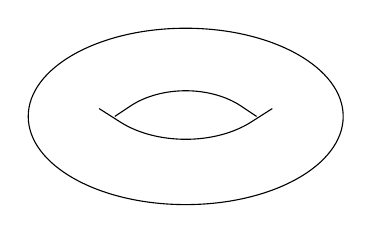
\begin{tikzpicture}
        \begin{scope}[shift={(5.5, 0)}]
            \draw (0,0) ellipse (2 and 1.12);
            \path[rounded corners=24pt] (-.9,0)--(0,.6)--(.9,0) (-.9,0)--(0,-.56)--(.9,0);
            \draw[rounded corners=28pt] (-1.1,.1)--(0,-.6)--(1.1,.1);
            \draw[rounded corners=24pt] (-.9,0)--(0,.6)--(.9,0);
          \end{scope}
        \end{tikzpicture}
        \end{minipage}
    \end{figure}
\end{itemize}
\end{exs}

Note that our definition of product topology is rather similar to the definition of open sets for metrics. We have a special class of subsets of the form $V\times W$, and a subset $U$ is open iff every point $x\in U$ is contained in some $V\times W\subseteq U$. In some sense, these subsets ``generate" the open sets.

Alternatively, if $U\subseteq X\times Y$ is open, then
\[
U=\bigcup_{(x,y)\in U}V_x\times W_y\,,
\]
i.e. $U\subseteq X\times Y$ is open iff it is a union of members of our special class of subsets. We call this special class the \emph{basis}.

\begin{defn}[Basis]
    Let $\mathcal{U}$ be topology on $X$. A subset $\mathcal{B}\subseteq\mathcal{U}$ is a \emph{basis} if ``$U\in \mathcal{U}$ iff $U$ is a union of sets in $\mathcal{B}$".
\end{defn}

\begin{exs}
\leavevmode
\begin{itemize}
    \item $\{V\times W:V\subseteq X,W\subseteq Y \text{are open}\}$ is a basis for the product topology on $X\times Y$.
    \item If $(X,d)$ is metric space, then
    \[
    \{B_{1/n}(x):n\in\mathbb{N}^+,x\in X\}
    \]
    is a basis for the topology induced by $d$.
\end{itemize}
\end{exs}

\subsubsection{Quotient topology}
If $X$ is a set and $\sim$ is an equivalence relation on $X$, then the quotient $X/\sim$ is the set of equivalence classes. The projection $\pi:X\rightarrow X/\sim$ is defined as $\pi(x)=[x]$, the equivalence class containing $x$.

\begin{defn}[Quotient topology]
    If $X$ is topological space, the \emph{quotient topology on} $X/\sim$ is given by: $U$ open in $X/\sim$ if $\pi^{-1}(U)$ open in $X$.
\end{defn}

We can think of the quotient as ``gluing" the points identified by $\sim$ together. The defining property is that $f:X/\sim\rightarrow Y$ is continuous iff $f\circ\pi:X\rightarrow Y$ is continuous.


\begin{exs}
\leavevmode
\begin{itemize}
    \item Let $X=\mathbb{R}$, $x\sim y$ iff $x-y\in\mathbb{Z}$. Then $X/\sim=\mathbb{R}/\mathbb{Z}\simeq S^1$, given by $[x]\mapsto(\cos 2\pi x,\sin2\pi x)$.
    \item Let $X=\mathbb{R}^2$, $\mathbf{v}\sim\mathbf{w}$ iff $\mathbf{v}-\mathbf{w}\in\mathbb{Z}^2$. Then $X/\sim=\mathbb{R}^2/\mathbb{Z}^2=(\mathbb{R}/\mathbb{Z})\times(\mathbb{R}/\mathbb{Z})\simeq S^1\times S^1=T^2$. Similarly, $\mathbb{R}^n/\mathbb{Z}^n=T^n=S^1\times S^1\times...\times S^1$.
    \item If $A\subseteq X$, define $\sim$ by $x\sim y$ iff $x=y$ or $x,y\in A$. This glues everything in $A$ together and leaves everything else alone. Note that we often write this as $X/A$, which is not consistent with the notation used above...
    \begin{itemize}
        \item Let $X=[0,1]$ and $A=\{0,1\}$. Then $X/A\sim S^1$ by, say $t\mapsto(\cos2\pi t,\sin2\pi t)$. Intuitively, the equivalence relation says that the two end points of $[0,1]$ are ``the same". So we join the ends together to get a circle.
        \begin{figure}[h]
            \centering
            \begin{minipage}{.47\textwidth}
            \centering
            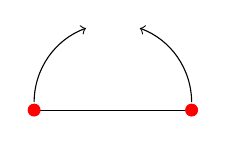
\begin{tikzpicture}
                \draw (-1, 0) node [circ,red] {} -- (1, 0) node [circ,red] {};
                \draw [->] (1, 0.1) arc (0:70:1);
                \draw [->] (-1, 0.1) arc (180:110:1);
            \end{tikzpicture}
            \end{minipage}
            \LARGE$\rightarrow$
            \begin{minipage}{.47\textwidth}
            \centering
            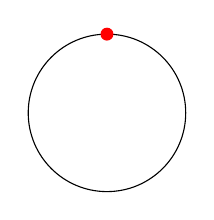
\begin{tikzpicture}
                \draw circle [radius=1];
                \node at (0, 1) [circ,red] {};
            \end{tikzpicture}
            \end{minipage}
        \end{figure}
        
        \item Let $X=D^n$ and $A=S^{n-1}$. Then $X/A\sim S^n$. This can be pictured as pulling the boundary of the disk together to a point to create a closed surface.
        
        \begin{figure}[h]
            \centering
            \begin{minipage}{.47\textwidth}
            \centering
            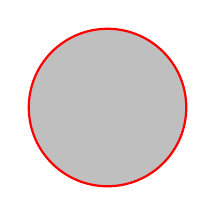
\begin{tikzpicture}
                \draw[thick, red, fill=gray!50!white] circle [radius=1];
            \end{tikzpicture}
            \end{minipage}
            \LARGE$\rightarrow$
            \begin{minipage}{.47\textwidth}
            \centering
            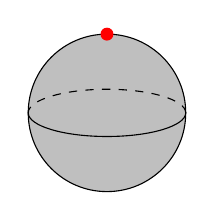
\begin{tikzpicture}
                \draw [fill=gray!50!white] (4, 0) circle [radius=1];
                \draw [dashed] (5, 0) arc (0:180:1 and 0.3);
                \draw (3, 0) arc (180:360:1 and 0.3);
                \node at (4, 1) [circ, red] {};
            \end{tikzpicture}
            \end{minipage}
        \end{figure}
    \end{itemize}
    \item Let $X=[0,1]\times[0,1]$ with $\sim$ given by $(0,y)\sim(1,y)$ and $(x,0)\sim(x,1)$. Then $X/\sim\,\simeq S^1\times S^1=T^2$ by, say
        \[
        (x,y)\mapsto\left((\cos2\pi x,\sin2\pi x),(\cos2\pi y,\sin2\pi y)\right)\,.
        \]
        Similarly, $T^3=[0,1]^3/\sim$, where the equivalence is analogous to that above.
        
        \begin{figure}[h]
            \centering
            \begin{minipage}{.47\textwidth}
            \centering
            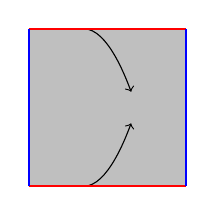
\begin{tikzpicture}
                \fill [thick, gray!50!white] (-1, -1) rectangle (1, 1);
                \draw [->] (-0.3, 1) parabola (0.3, 0.2);
                \draw [->] (-0.3, -1) parabola (0.3, -0.2);
                \draw [thick, red] (-1, -1) -- (1, -1);
                \draw [thick, red] (-1, 1) -- (1, 1);
                \draw [thick, blue] (-1, -1) -- (-1, 1);
                \draw [thick, blue] (1, -1) -- (1, 1);
            \end{tikzpicture}
            \end{minipage}
            \LARGE$\rightarrow$
            \begin{minipage}{.47\textwidth}
            \centering
            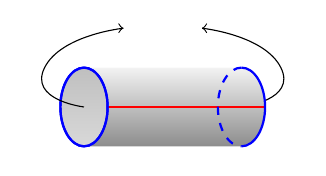
\begin{tikzpicture}
                \draw plot [smooth, tension=1.5] coordinates {(1, 0) (1.5, 0.5) (0.5, 1)};
                \shade [bottom color=gray!90!white, top color = gray!10!white] (-1, 0.5) arc (90:-90:0.3 and 0.5) -- (1, -0.5) arc (-90:90:0.3 and 0.5) -- cycle;
                \shade [bottom color=gray!30!white, top color = gray!50!white] (-1, 0) circle [x radius = 0.3, y radius = 0.5];
                \draw [thick, red] (-0.7, 0) -- (1.3, 0);
                \draw [thick, blue] (-1, 0) circle [x radius = 0.3, y radius = 0.5];
                \draw [thick, blue] (-1, 0.5) arc (90:-90:0.3 and 0.5);
                \draw [thick, blue] (1, -0.5) arc (-90:90:0.3 and 0.5);
                \draw [thick, blue] (-1, 0.5) arc (90:270:0.3 and 0.5);
                \draw [dashed, thick, blue] (1, 0.5) arc (90:270:0.3 and 0.5);
                \draw plot [smooth, tension=1.5] coordinates {(-1, 0) (-1.5, 0.5) (-0.5, 1)};
                \draw [->] (-0.51, 1) -- (-0.5, 1);
                \draw [->] (0.51, 1) -- (0.5, 1);
            \end{tikzpicture}
            \end{minipage}
        \end{figure}
\end{itemize}
\end{exs}

Note that even if $X$ is Hausdorff, $X/\sim$ may not be. For example, $\mathbb{R}/\mathbb{Q}$ is not Hausdorff.

\section{Connectedness}
\begin{defn}[Connected space]
    A topological space $X$ is \emph{disconnected} if $X$ can be written as $A\cup B$, where $A$, $B$ are disjoint, non-empty open subsets of $X$. We then say $A$, $B$ disconnect $X$. A space is \emph{connected} if it is not disconnected.
\end{defn}

Note that being connected is a property of a \emph{space}, not a subset. When we say ``$A$ is connected subset of $X$", it means that $A$ is connected with subspace topology inherited from $X$.

Being (dis)connected is a topological property, i.e. if $X$ is (dis)connected, and $X\simeq Y$, then $Y$ is (dis)connected. To show this, let $f:X\rightarrow Y$ be the homeomorphism. By definition, $A$ is open in $X$ iff $f(A)$ is open in $Y$. So $A$ and $B$ disconnect $X$ iff $f(A)$ and $f(B)$ disconnect $Y$.

\begin{exs}
\leavevmode
\begin{itemize}
    \item If $X$ has the coarse topology, it is connected.
    \item If $X$ has the discrete topology and at least 2 elements, it is disconnected.
    \item Let $X\subseteq \mathbb{R}$. If $\exists\alpha\in\mathbb{R\setminus X}$ s.t. there is some $a,b\in X$ with $a<\alpha<b$, then $X$ is disconnected. In particular, $X\cap(-\infty,a)$ and $X\cap(a,\infty)$ disconnect $X$.\\
    For example, $(0,1)\cup(1,2)$ is disconnected.
\end{itemize}
\end{exs}

\begin{prop}
    $X$ is disconnected iff exists a continuous surjective $f:X\rightarrow\{0,1\}$ with the discrete topology.
    
    Alternatively, $X$ is disconnected iff any continuous map $f:X\rightarrow\{0,1\}$ is constant.
\end{prop}
\begin{proof}
$(\Rightarrow)$ If $A$, $B$ disconnect $X$, define
\[
f(x)=\left\{\begin{array}{lr}
    0\quad & x\in A \\
    1\quad & x\in B
\end{array}\right.
\]

Then $f^{-1}(\emptyset)$, $f^{-1}(\{0,1\})=X$, $f^{-1}(\{0\})=A$ and $f^{-1}(\{1\})=B$ are all open, so $f$ continuous. Since $A, B$ non-empty, $f$ is also surjective.\\
$(\Leftarrow)$ Given $f:X\mapsto\{0,1\}$ surjective and continuous, define $A=f^{-1}(\{0\})$, $B=f^{-1}(\{1\})$. Then $A$ and $B$ disconnect $X$.
\end{proof}

\begin{thm}
$[0,1]$ is connected.
\end{thm}

\begin{proof}
Note that $\mathbb{Q}\cup[0,1]$ is disconnected, since we can pick any irrational number $a$, then $\{x:x<a\}$ and $\{x:x>a\}$ disconnect the interval. So we need to use a special property of $\mathbb{R}$, in that every non-empty $A\subseteq[0,1]$ has a supremum.

So suppose $A$, $B$ disconnect $[0,1]$. Wlog assume $1\in B$. Since $A$ is non-empty, $\alpha=\sup A$ exists. Then either
\begin{itemize}
    \item $\alpha\in A$: so $\alpha<1$ since $1\in B$. $A$ is open, which means $\exists\varepsilon>0$ s.t. $B_\varepsilon(\alpha)\subseteq A$. Then $\alpha+\varepsilon/2\in A$, contradicting the supremumality of $\alpha$.
    \item $\alpha\notin A$: so $\alpha\in B$. Since $B$ is open, $\exists\varepsilon>0$ s.t. $B_\varepsilon(\alpha)\subseteq B$. Then $a\leq\alpha-\varepsilon\;\forall a\in A$, which contradicts the fact that $\alpha$ must be the least upper bound of $A$.
\end{itemize}
So $A$, $B$ cannot exist and $[0,1]$ is continuous.
\end{proof}

\begin{prop}
    If $f:X\rightarrow Y$ is continuous and $X$ is connected, then $\im f$ is also connected.
\end{prop}

\begin{proof}
If $\im f$ is not connected, let $g:\im f\rightarrow\{0,1\}$ be continuous surjective. Then $g\circ f:X\rightarrow\{0,1\}$ is continuous surjective. So by previous proposition, $X$ is disconnected, a contradiction.
\end{proof}

\begin{thm}[Intermediate value theorem]
Suppose $f:X\rightarrow\mathbb{R}$ continuous and $X$ connected. If $\exists x_0,x_1$ s.t. $f(x_0)<0<f(x_1)$, then $\exists x\in X$ s.t. $f(x)=0$.
\end{thm}

\begin{proof}
Suppose no such $x$ exists. Then $0\notin \im f$ while $0>f(x_0)\in\im f$, $0<f(x_1)\in\im f$. Then $\im f$ disconnected, which from our previous proposition means $X$ disconnected, a contradiction.

Alternatively, if $f(x)\neq0\;\forall x$, then $\frac{f(x)}{|f(x)|}$ is a continuous surjection from $X$ to $\{-1,1\}$, which gives a contradiction.
\end{proof}

\begin{cor}
If $f:[0,1]\rightarrow\mathbb{R}$ continuous with $f(0)<0<f(1)$, then $\exists x\in[0,1]$ with $f(x)=0$.
\end{cor}

Note that the converse to the intermediate value theorem is also true: if $X$ disconnected, we can find $f:X\rightarrow\{0,1\}$ that is continuous. Then the function $g(x)=f(x)-\frac{1}{2}$ does not satisfy the intermediate value property.

\subsection{Path connectedness}
\begin{defn}[Path]
    Let $X$ be topological space, and $x_0, x_1\in X$. Then a path from $x_0$ to $x_1$ is a continuous function $\gamma:[0,1]\mapsto X$ s.t. $\gamma(0)=x_0$, $\gamma(1)=x_1$.
\end{defn}

A space is path connected if we can join any two points with a path.

\begin{defn}[Path connectedness]
    A topological space $X$ is \emph{path connected} if for all points $x_0, x_1\in X$, there exists a path from $x_0$ to $x_1$.
\end{defn}

\begin{exs}
\leavevmode
\begin{itemize}
    \item $(a,b)$, $[a,b)$, $(a,b]$, $\mathbb{R}$ are all path connected (using paths given by linear functions)
    \item $\mathbb{R}^n$ is path connected (e.g. using $\gamma(t)=t\mathbf{x}_1+(1-t)\mathbf{x}_0$)
    \item $\mathbb{R}\setminus\{0\}$ is path-connected for $n>1$, using line segments or bent line segments around the hole. 
\end{itemize}
\end{exs}

Path connectedness is a stronger property than connectedness.

\begin{prop}
    If $X$ is path connected, then it is also connected.
\end{prop}

\begin{proof}
Let $X$ be path connected, and let $f:X\rightarrow\{0,1\}$ be continuous. Let $x,y\in X$. Path connectedness of $X$ means that $\exists$ map $\gamma:[0,1]\rightarrow X$ s.t. $\gamma(0)=x$, $\gamma(1)=y$. Then the map $f\circ\gamma:[0,1]\rightarrow\{0,1\}$ must be constant, since $[0,1]$ is connected. In particular $f(\gamma(0))=f(\gamma(1))$, or $f(x)=f(y)$. Since this is for arbitrary $x,y$, $f$ must be constant.
\end{proof}

\begin{lem}
    Suppose $f:X\rightarrow Y$ is a homeomorphism and $A\subseteq X$. Then $f|_A:A\rightarrow f(A)$ is a homeomorphism.
\end{lem}

\begin{proof}
Since $f$ is bijection, $f|_A$ is also bijection. If $U\subseteq f(A)$ open, then $U=f(A)\cap U'$ for some $U'$ open in $Y$. So $f|_A^{-1}(U)=f^{-1}(U')\cap A$ is open in $A$. So $f|_A$ continuous. Similarly, we can show that $f|_A^{-1}$ is continuous.
\end{proof}

\begin{ex}
$[0,1]\not\simeq(0,1)$. Suppose it were. Let $f:[0,1]$ be homeomorphism, $A=(0,1]$. Then $f|_A:(0,1]\rightarrow(0,1)\setminus\{f(0)\}$ is homeomorphism. But $(0,1]$ connected and $(0,1]\setminus\{f(0)\}$ disconnected, a contradiction.

Similarly, $[0,1)\not\simeq [0,1]$ and $[0,1)\not\simeq(0,1)$. Also, $\mathbb{R}^n\not\simeq \mathbb{R}$ for $n>1$, and $S^1$ is not homeomorphic to any subset of $\mathbb{R}$.
\end{ex}

\subsubsection{Higher connectedness*}

\subsection{Components}
If a space is disconnected, we may try to divide the space into several components, each of which is (maximally) connected. We will have different notions of components for each type of connectedness.

\subsubsection{Path components}
\begin{lem}
    Define $x\sim y$ if there is a path from $x$ to $y$ in $X$. Then $\sim$ is an equivalence relation.
\end{lem}

\begin{proof}
\leavevmode
\begin{enumerate}
    \item For any $x\in X$, let $\gamma_x:[0,1]\rightarrow X$ be $\gamma(t)=x$, the constant path. Then this is a path from $x$ to $x$, so $x\sim x$.
    \item If $\gamma:[0,1]\rightarrow X$ is path from $x$ to $y$, then $\bar{\gamma}:[0,1]\rightarrow X$ by $t\mapsto\gamma(1-t)$ is path from $y$ to $x$. So $x\sim y\Rightarrow y\sim x$.
    \item If $\gamma_1$ is path from $x$ to $y$, $\gamma_2$ path from $y$ to $z$, then $\gamma_2*\gamma_1$ defined by
    \[
    t\mapsto\left\{\begin{array}{lr}
        \gamma_1(2t)\quad & t\in[0,1/2] \\
        \gamma_2(2t-1)\quad & t\in[1/2,1]
    \end{array}\right.
    \] is path from $x$ to $z$. So $x\sim y$, $y\sim z$ implies $x\sim z$.
    \end{enumerate}
\end{proof}

This lemma then allows us to define the path components.
\begin{defn}[Path components]
    Equivalence classes of the relation ``$x\sim y$ if there is a path from $x$ to $y$" are \emph{path components} of $X$.
\end{defn}

\subsubsection{Connected components}
These are components wrt regular connectedness.
\begin{prop}
    Suppose $Y_\alpha\subseteq X$ is connected $\forall\alpha\in T$ and that $\bigcap_{\alpha\in T}Y_\alpha\neq\emptyset$. Then $Y=\bigcup_{\alpha\in T}Y_\alpha$ is connected.
\end{prop}

\begin{proof}
Suppose the contrary that $A$, $B$ disconnect $Y$. Then $A$, $B$ open in $Y$, and $A=Y\cap A'$, $B=Y\cap B'$ for $A',B'$ open in $X$. Let
\begin{equation}
    A_\alpha=Y_\alpha\cap A=Y_\alpha\cap A'\,,\quad B_\alpha=Y_\alpha\cap B=Y_\alpha\cap B'\,,
\end{equation}
where $\alpha$ is fixed. Then $A_\alpha, B_\alpha$ open in $Y_\alpha$. Since $Y=A\cup B$,
\begin{equation}
    Y_\alpha=Y\cap Y_\alpha=(A\cup B)\cap Y_\alpha=A_\alpha\cup B_\alpha\,.
\end{equation}
Also $A\cap B=\emptyset$, which means $A_\alpha\cap B_\alpha=Y_\alpha\cap(A\cap B)=\emptyset$. So $A_\alpha,B_\alpha$ disjoint. But $Y_\alpha$ is connected, so this means either $A_\alpha$ or $B_\alpha$ is the empty set.

By assumption, $\bigcap_{\alpha\in T}Y_\alpha\neq\emptyset$, so pick $y\in\bigcap_{\alpha\in T}Y_\alpha$. Then $y$ is in either $A$ or $B$. Wlog assume $y\in A$, then $y\in Y_\alpha\;\forall\alpha\Rightarrow y\in A_\alpha\;\forall\alpha$. So $A_\alpha\neq\emptyset\;\forall\alpha$, which makes $B_a$ empty for all $\alpha$. So $B=\emptyset$.

This means that $A$ and $B$ do not disconnect $Y$ after all, a contradiction.
\end{proof}

This allows us to define the connected components as follows:

\begin{defn}[Connected component]
    If $x\in X$, define
    \begin{equation}
        \mathcal{C}(x)=\{A\subseteq X:x\in A\text{ and }A\text{ connected}\}\,,
    \end{equation}
    then 
    \begin{equation}
        C(x)=\bigcup_{A\in\mathcal{C}(x)}A
    \end{equation}
    is the \emph{connected component} of $x$.
\end{defn}

Note that $C(x)$ is the largest connected subset of $X$ containing $x$. To show this, first note that $\{x\}\in\mathcal{C}(x)$. So $x\in C(x)$. Also $x\in\bigcap_{A\in \mathcal{C}(x)} A$, so $\bigcap_{A\in\mathcal{C}(x)}A\neq\emptyset$, and by our previous proposition this implies that $C(x)$ is connected.

\begin{lem}
    If $y\in C(x)$, then $C(y)=C(x)$.
\end{lem}

\begin{proof}
Since $y\in C(x)$ and $C(x)$ connected, $C(x)\subseteq C(y)$. So $x\in C(y)$. Then $C(y)\subseteq C(x)$, i.e. $C(y)=C(x)$.
\end{proof}

It follows that $x\sim y$ if $x\in C(y)$ is an equivalence relation and the connected components of $X$ are the equivalence classes.

\begin{exs}
\leavevmode
\begin{itemize}
    \item Let $X=(-\infty,0)\cup(0,\infty)\subseteq\mathbb{R}$. Then the connected components are $(-\infty,0)$ and $(0,\infty)$, which are also path components.
    \item Let $X=\mathbb{Q}\subseteq\mathbb{R}$. Then $C(x)=\{x\}\;\forall x\in X$. In this case, we say that $X$ is totally disconnected.
\end{itemize}
\end{exs}

Note that $C(x)$ and $X\setminus C(x)$ need not disconnect $X$, even though it is the case in the first example. Disconnection requires $C(x)$ and $X\setminus C(x)$ to be open, in which $C(x)=\{x\}$ in the second example is not, for example.

Path components need not equal the connected components, but rather since path connected spaces are connected, are subsets of the connected components.

\begin{ex}
Let $Y=\{(0,y):y\in\mathbb{R}\subseteq\mathbb{R}^2$ be the $y$ axis, and let $Z=\{(x,\frac{1}{x}\sin\left(\frac{1}{x}\right):x\in(0,\infty)\}$. 

Let $X=Y\cup Z\subseteq\mathbb{R}^2$. We claim that $X$ and $Y$ are path components of $X$. Since $Y$, $Z$ individually path connected, we only need to show that there is no continuous $\gamma:[0,1]\rightarrow X$ with $\gamma(0)=(0,0)$, $\gamma(1)=(1,\sin 1)$.
\end{ex}


There are special cases where connected subsets are also path-connected.

\begin{prop}
    If $U\subseteq\mathbb{R}^n$ open and connected, then it is also path-connected.
\end{prop}

\begin{proof}
Let $A$ be path component of $U$. Let $a\in A$. Since $U$ open, $\exists\varepsilon>0$ s.t. $B_\varepsilon(a)\subseteq U$. Now $B_\varepsilon(a)\simeq\Int(D^n)$ is path-connected (e.g. use line segments connecting the points), and since $A$ is path component with $a\in A$, we have $B_\varepsilon(a)\subseteq A$. So $A$ is open subset of $U$.

Now suppose $b\in U\setminus A$. Then since $U$ open, $\exists\varepsilon>0$ s.t. $B_\varepsilon(b)\subseteq U$. $B_\varepsilon(b)$ is path-connected, so if $B_\varepsilon(b)\cap A\neq\emptyset$, then $B_\varepsilon(b)\subseteq A$. But this implies $b\in A$, a contradiction. So $B_\varepsilon(b)\cap A=\emptyset$, which means $B_\varepsilon(b)\subseteq U\setminus A$. So $U\setminus A$ is open.

These two results give $A$, $U\setminus A$ as disjoint open subsets of $U$. Since $U$ is connected, we require $U\setminus A=\emptyset$, or that $U=A$. So $U$ is path-connected.
\end{proof}

\section{Compactness}
\begin{defn}[Open cover]
    Let $\mathcal{U}\subseteq\mathbb{P}(X)$ be topology on $X$. An \emph{open cover} of $X$ is a subset $\mathcal{V}\subseteq\mathcal{U}$ s.t.
    \begin{equation}
        \bigcup_{V\in\mathcal{V}}V=X\,.
    \end{equation}
    We then say $\mathcal{V}$ covers $X$.
    
    If $\mathcal{V}'\subseteq\mathcal{V}$ and $\mathcal{V}'$ covers $X$, then $\mathcal{V}'$ is a \emph{subcover} of $\mathcal{V}$.
\end{defn}

\begin{defn}[Compact space]
    A topological space $X$ is \emph{compact} if every open cover $\mathcal{V}$ of $X$ has a finite subcover $\mathcal{V}'=\{V_1,...,V_n\}\subseteq\mathcal{V}$.
\end{defn}

The definition of compactness may seem strange and unintuitive at first, only because we have yet encountered such an idea before. The notion of compactness can be seen as a generalisation of being ``closed and bounded" in $\mathbb{R}$, or as a generalisation of finiteness. Its relation to these more familiar properties will be shown below.

\begin{exs}
\leavevmode
\begin{itemize}
    \item If $X$ is finite, then $\mathbb{P}(X)$ is finite. So any open cover of $X$ is finite, i.e. $X$ is compact.
    \item Let $X=\mathbb{R}$ and $\mathcal{V}=\{(-R,R):R\in\mathbb{R},R>0\}$. This is an open cover with no finite subcover, so $\mathbb{R}$ is not compact. Hence all open intervals are not compact since they are homeomorphic to $\mathbb{R}$.
    \item Let $X=[0,1]\cap\mathbb{Q}$. Let
    \begin{equation}
        U_n=X\setminus(\alpha-1/n,\alpha+1/n)\,,
    \end{equation}
    for some irrational $\alpha\in(0,1)$ (e.g. $\alpha=1/\sqrt{2}$). Then $\bigcup_{n>0}U_n=X$ since $\alpha$ is irrational. Then $\mathcal{V}=\{U_n:n\in\mathbb{Z}>0\}$ is open cover of $X$. This has no finite subcover, so $X$ is not compact.
\end{itemize}
\end{exs}

\begin{thm}
$[0,1]$ is compact.
\end{thm}

\begin{proof}
Like before, $[0,1]\cap\mathbb{Q}$ is not compact, so we need to use a special property of the reals. Suppose $\mathcal{V}$ is open cover of $[0,1]$. Let
\begin{equation}
    A=\{a\in[0,1]:[0,a]\text{ has finite subcover of }\mathcal{V}\}\,.
\end{equation}
We first show that this is non-empty. Since $\mathcal{V}$ covers $[0,1]$, there is some $V_0$ that contains $0$. So $\{0\}$ has finite subcover $V_0$, which means $0\in A$.

Now note that by definition, if $0\leq b\leq a$ and $a\in A$, then $b\in A$. 

Let $\alpha=\sup A$. Suppose $\alpha<1$. Then $\alpha\in[0,1]$. Let $\alpha\in V_\alpha$. This is open, so there is some $\varepsilon$ s.t. $B_\varepsilon(\alpha)\subseteq V_\alpha$. By definition of $\alpha$, we must then have $\alpha-\varepsilon/2\in A$. So $[0,\alpha-\varepsilon/2]$ has finite subcover. Adding $V_\alpha$ to that subcover gives a finite subcover of $[0,\alpha+\varepsilon/2]$, contradiction. So $\alpha=\sup A=1$.

So $\exists V_1\in\mathcal{V}$ s.t. $1\in V_1$ and $\exists\varepsilon>0$ with $(1-\varepsilon,1]\subseteq V_1$. $1-\varepsilon\in A$, so exists finite $\mathcal{V}'\subseteq\mathcal{V}$ which covers $[0,1-\varepsilon/2]$. So $\mathcal{W}=\mathcal{V}'\cup \{V_1\}$ is a finite subcover of $\mathcal{V}$.
\end{proof}

The following proposition shows how compactness is related to closedness.

\begin{prop}
    If $X$ is compact and $C$ is closed subset of $X$, then $C$ is also compact.
\end{prop}

\begin{proof}
    To prove this, given an open cover of $C$, we need to find a finite subcover. First convert this into an open cover of $X$, by adding $X\setminus C$, which is open since $C$ is closed. Then since $X$ compact, there is a finite subcover of this, which we can then convert back to a subcover of $C$.
    
    Formally, suppose $\mathcal{V}$ is open cover of $C$. Say $\mathcal{V}=\{V_\alpha:\alpha\in T\}$. For each $\alpha$, $V_\alpha$ is open in $C$, so $V_\alpha=C\cup V_\alpha'$ for some $V_\alpha'$ open in $X$. Also, since $\bigcup_{\alpha\in T}V_a=C$, we have $\bigcup_{\alpha\in T}V_a'\supseteq C$.
    
    So since $C$ closed, $U=X\setminus C$ is open in $X$, which means $\mathcal{W}=\{V_\alpha':\alpha\in T\}\cup\{U\}$ is an open cover of $X$. $X$ is compact, so $\mathcal{W}$ has finite subcover $\mathcal{W}'=\{V_{\alpha_1}',...,V_{\alpha_n}',U\}$. $U\cap C=\emptyset$, so $\{V_{\alpha_1},...,V_{\alpha_n}\}$ is finite subcover of $C$.
\end{proof}

The converse is not always true, but holds for Hausdorff spaces.

\begin{prop}
    Let $X$ be Hausdorff space. If $C\subseteq X$ compact, then $C$ is closed in $X$.
\end{prop}

\begin{proof}
    Let $U=X\setminus C$. We show that $U$ is open. This is done by showing that for any $x$, $\exists U_x\subseteq U$, $x\in U_x$. Then $U=\bigcup_{x\in U} U_x$ is open since it is a union of open sets.
    
    To show that such a $U_x$ exists, first fix $x\in U$. Since $X$ is Hausdorff, for each $y\in C\;\exists U_{xy}, W_{xy}$ open nhoods of $x$, $y$ respectively with $U_{xy}\cap W_{xy}=\emptyset$.
    
    Then $\mathcal{W}=\{W_{xy}\cap C:y\in C\}$ is open cover of $C$. Since $C$ compact, exists finite subcover $\mathcal{W}'=\{W_{xy_1}\cap C,...,W_{xy_n}\cap C\}$.
    
    Now let $U_x=\bigcap_{i=1}^n U_{xy_i}$. Then $U_x$ open since it is a finite intersection of open sets. Finally note that $W_x=\bigcup_{i=1}^nW_{xy_i}\supseteq C$ since $\{W_{xy_i}\cap C\}$ is open cover, with $W_x\cap U_x=\emptyset$. So $U_x\subseteq U$ as required.
    
    \begin{figure}[t]
        \centering
        \includegraphics[width=0.5\textwidth]{fig1.PNG}
        \caption{Open neighbourhoods of $x\in X\setminus C$, and $y\in C$.}
        \label{fig:fig1}
    \end{figure}
\end{proof}

We now relate compactness to boundedness. We first need to define it for general metric spaces:
\begin{defn}[Bounded metric space]
    A metric space $(X,d)$ is \emph{bounded} if $\exists M\in\mathbb{R}$ s.t. $d(x,y)\leq M\;\forall x,y\in X$.
\end{defn}

\begin{ex}
$A\subseteq\mathbb{R}$ is bounded iff $A\subseteq[-N,N]$ for some $N\in\mathbb{R}$.
\end{ex}

Note that boundedness is \emph{not} a topological property. For example, $(0,1)\simeq\mathbb{R}$ but $(0,1)$ is bounded while $\mathbb{R}$ is not. It depends on the metric $d$, not just the topology it induces.

\begin{prop}
    A compact metric space $(X,d)$ is bounded.
\end{prop}

\begin{proof}
    Pick $x\in X$. Then $V=\{B_r(x):r\in\mathbb{R}^+\}$ is open cover of $X$. Since $X$ is compact, there is a finite subcover $\{B_{r_1}(x),...,B_{r_n}(x)\}$. Let $R=\max\{r_1,...,r_n\}$. Then $d(x,y)<R\;\forall y\in X$. So $\forall y,z\in X$, 
    \begin{equation}
        d(y,z)\leq d(y,x)+d(x,z) <2R\,.
    \end{equation}
    So $X$ is bounded.
\end{proof}

\begin{thm}[Heine-Borel]
$C\subseteq\mathbb{R}$ is compact iff $C$ is closed and bounded.
\end{thm}

\begin{proof}
    Since $\mathbb{R}$ is a metric space (and hence Hausdorff), $C$ is also a metric space. So if $C$ compact, then by the previous two propositions it is also closed in $\mathbb{R}$ and bounded.
    
    Conversely if $C$ is closed and bounded, then $C\subseteq[-N,N]$ for some $N\in\mathbb{R}$. Now $[-N,N]\simeq[0,1]$ is compact, and $C=C\cap[-N,N]$ is closed in $[-N,N]$, so $C$ is compact.
\end{proof}

\begin{cor}
If $A\subseteq\mathbb{R}$ compact, $\exists\alpha\in A$ s.t. $\alpha\geq a\;\forall a\in A$.
\end{cor}

\begin{proof}
    Since $A$ is compact, it is bounded. Then by definition $\alpha=\sup A\geq a\;\forall a\in A$. So we need to show that $\alpha\in A$.
    
    Suppose $\alpha\notin A$. Then $\alpha\in\mathbb{R}\setminus A$. Since $A$ is compact, it is closed in $\mathbb{R}$. So $\mathbb{R}\setminus A$ is open. Then $\exists\varepsilon>0$ s.t. $B_\varepsilon(\alpha)\subseteq\mathbb{R}\setminus A$, which implies that $a\leq\alpha-\varepsilon\;\forall a\in A$, contradicting the assumption that $\alpha=\sup A$. So $\alpha\in A$.
\end{proof}

We call $\alpha=\max A$ the maximum element of $A$.

Previously, we proved that if $X$ connected and $f:X \rightarrow Y$, then $\im f\subseteq Y$ is connected. The same is true for compactness.
\begin{prop}
    If $f:X\rightarrow Y$ continuous and $X$ compact, then $\im f\subseteq Y$ is also compact.
\end{prop}

\begin{proof}
    Suppose $\mathcal{V}=\{V_\alpha:\alpha\in T\}$ is open cover of $\im f$. Since $V_\alpha$ open in $\im f$, $V_\alpha=\im f\cap V_\alpha'$ for some $V_\alpha'$ open in $Y$. Then
    \begin{equation}
        W_\alpha=f^{-1}(V_\alpha)=f^{-1}(V_\alpha')
    \end{equation}
    is open in $X$. If $x\in X$ then $f(x)\in V_\alpha$ for some $\alpha$, i.e. $x\in W_\alpha$. Thus $\mathcal{W}=\{W_\alpha:\alpha\in T\}$ is open cover of $X$.
    
    Since $X$ compact, there is finite subcover $\{W_{\alpha_1},...,W_{\alpha_n}\}$ of $\mathcal{W}$; since $V_\alpha\subseteq\im f$, $f(W_\alpha)=f(f^{-1}(V_\alpha))=V_\alpha$. So $\{V_{\alpha_1},...,V_{\alpha_n}\}$ is a finite subcover of $\mathcal{V}$.
\end{proof}

\begin{thm}[Maximum value theorem]
If $f:X\rightarrow\mathbb{R}$ continuous and $X$ compact, then $\exists x\in X$ s.t. $f(x)\geq f(y)\;\forall y\in X$.
\end{thm}

\begin{proof}
    Since $X$ compact, $\im f$ is compact. Let $\alpha=\max\{\im f\}$. Then $\alpha\in\im f$. So $\exists x\in X$ s.t. $f(x)=\alpha$. Then by definition $f(x)\geq f(y)\;\forall y\in X$.
\end{proof}

\begin{cor}
If $f:[0,1]\rightarrow\mathbb{R}$ continuous, then $\exists x\in[0,1]$ s.t. $f(x)\geq f(y)\;\forall y\in[0,1]$.
\end{cor}

\begin{proof}
    Result follows using maximum value theorem since $[0,1]$ is compact.
\end{proof}

\subsection{Compactness of product spaces}
Recall the product topology on $X\times Y$: $U\subseteq X\times Y$ is open if it is a union of sets of the form $V\times W$ s.t. $V\subseteq X$, $W\subseteq Y$ are open.

\begin{thm}
If $X$, $Y$ are compact, then so is $X\times Y$.

\begin{proof}
    First consider the special type of open cover $\mathcal{V}$ of $X\times Y$ s.t. every $U\in\mathcal{V}$ has the form $U=V\times W$, where $V\subseteq X$ and $W\subseteq Y$ open. For every $(x,y)\in X\times Y$, $\exists U_{xy}\in\mathcal{V}$ s.t. $(x,y)\in U_{xy}$. Write
    \[
    U_{xy}=V_{xy}\times W_{xy}\,,
    \]
    where $V_{xy}\subseteq X$, $W_{xy}\subseteq Y$ open, $x\in V_{xy}$, $y\in W_{xy}$.
    
    Now fix $x\in X$. Then $\mathcal{W}_x=\{W_{xy}:y\in Y\}$ is open cover of $Y$. Since $Y$ is compact, there is finite subcover $\{W_{xy_1},...,W_{xy_n}\}$. So $V_x=\bigcup^n_{i=1}V_{xy_i}$ is finite intersection of open sets, which is open in $X$. Moreover, $\mathcal{V}_x=\{U_{xy_1},...,U_{xy_n}\}$ covers $V_x\times Y$.
    
    \begin{figure}[h]
    \centering
        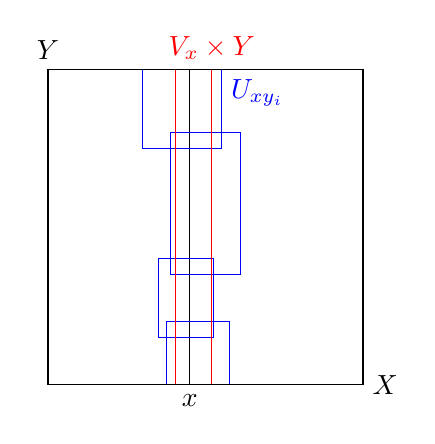
\begin{tikzpicture}
          \draw (1.8, 0) node [black, below] {$x$} -- (1.8, 4);
          \draw [blue] (1.5, 0) rectangle (2.3, .8);
          \draw [blue] (1.4, 0.6) rectangle (2.1, 1.6);
          \draw [blue] (1.55, 1.4) rectangle (2.45, 3.2);
          \draw [blue] (1.2, 3) rectangle (2.2, 4) node [anchor = north west] {$U_{xy_i}$};
    
          \draw [red] (1.62, 0) rectangle (2.08, 4) node [above] {$V_x\times Y$};
          \draw (0, 0) rectangle (4, 4);
          \node at (4, 0) [right] {$X$};
          \node at (0, 4) [above] {$Y$};
        \end{tikzpicture}
    \end{figure}
    
    Here $\mathcal{O}=\{V_x:x\in X\}$ is open cover of $X$. Since $X$ compact, there is finite cover $\{V_{x_1},...,V_{x_m}\}$. Then $\mathcal{V}'=\bigcup_{i=1}^m\mathcal{V}_{x_i}$ is finite subset of $\mathcal{V}$, which covers all of $X\times Y$.
    
    In the general case, suppose $\mathcal{V}$ is open cover of $X\times Y$. For each $(x,y)\in X\times Y$, $\exists U_{xy}\in\mathcal{V}$ s.t. $(x,y)\in U_{xy}$. Since $U_{xy}$ open, $\exists V_{xy}\in X, W_{xy}\subseteq Y$ open with $V_{xy}\times W_{xy}\subseteq U_{xy}$ and $x\in V_{xy},y\in W_{xy}$.
    
    Then $\mathbb{Q}=\{V_{xy}\times W_{xy}:(x,y)\in(X,Y)\}$ is open cover of $X\times Y$ of the type already considered above. So it has finite subcover $\{V_{x_1y_1}\times W_{x_1y_1},...,V_{x_ny_n}\times W_{x_ny_n}\}$. Also $V_{x_iy_i}\times W_{x_iy_i}\subseteq U_{x_iy_i}$. So $\{U_{x_1y_1},...,U_{x_ny_n}\}$ is finite subcover of $X\times Y$.
\end{proof}
\end{thm}

\begin{ex}
The unit cube $[0,1]^n=[0,1]\times[0,1]\times...\times[0,1]$ is compact.
\end{ex}

\begin{cor}[Heine-Borel in $\mathbb{R}^n$]
$C\subseteq\mathbb{R}^n$ is compact iff $C$ is closed and bounded.
\end{cor}

\begin{proof}
    If $C$ bounded, $C\subseteq[-N,N]^n$ for some $N\in\mathbb{R}$, which is compact. Remaining proof is exactly the same as for $n=1$. 
\end{proof}

\subsection{Compactness of quotient spaces}
It is easy to show that the quotient of a compact space is compact, since every open subset in the quotient space can be projected back to an open subset of the original space. Hence we can project an open cover from the quotient space to the original space, giving a finite subcover.

\begin{prop}
    Suppose $f:X\rightarrow Y$ is a continuous bijection. If $X$ is compact and $Y$ is Hausdorff, then $f$ is a homeomorphism.
\end{prop}

\begin{proof}
    We show that $f^{-1}$ is continuous. To do this, it suffices to show that $(f^{-1})^{-1}(C)$ is closed in $Y$ whenever $C$ is closed in $X$. Since $f$ is bijection, $(f^{-1})^{-1}(C)=f(C)$.
    
    Suppose $C$ closed in $X$. Since $X$ is compact, $C$ is also compact. Since $f$ is continuous, $f(C)=(\im f|_C)$ is compact. So if $Y$ Hausdorff and $f(C)\subseteq Y$ compact, $f(C)$ is closed.
\end{proof}

Now recall that if $\sim$ is equivalence relation on $X$, $\pi:X\rightarrow X/\sim$ is continuous iff $f\circ\pi:X\rightarrow Y$ continuous.

\begin{cor}
Suppose $f:X/\sim\,\rightarrow Y$ is a bijection, $X$ compact, $Y$ Hausdorff, and $f\circ\pi$ continuous. Then $f$ is a homeomorphism.
\end{cor}

\begin{proof}
    Since $X$ compact and $\pi:X\mapsto X/\sim$ continuous, $\im\pi\subseteq X/\sim$ is compact. Since $f\circ\pi$ continuous, $f$ continuous. Result follows from above proposition.
\end{proof}

\begin{ex}
Let $X=D^2$ and $A=S^1\subseteq X$. Then $f:X/A\rightarrow S^2$ by $(r,\theta)\mapsto(1,\pi r,\theta)$ in spherical coords is a homeomorphism. We can check that $f$ is continuous bijection and $D^2$ is compact. So $X/A\simeq S^2$.
\end{ex}

\subsection{Sequential compactness}

\begin{defn}[Sequential compactness]
    A topological space $X$ is \emph{sequentially compact} if every sequence $(x_n)$ in $X$ has convergent subsequence (that converges to a point in $X$).
\end{defn}

\begin{ex}
$(0,1)\subseteq\mathbb{R}$ is not sequential compact since no subsequence of $(1/n)$ converges to any of $x\in(0,1)$.
\end{ex}

\begin{lem}
    Let $(x_n)$ be sequence in metric space $(X,d)$ and $x\in X$. Then $(x_n)$ has subsequence converging to $x$ iff for every $\varepsilon>0$, $x_n\in B_\varepsilon(x)$ for infinitely many $n$.
\end{lem}

\begin{proof}
    $(\Rightarrow)$ If $(x_{n_i})\rightarrow x$, then for every $\varepsilon$, we can find $I$ s.t. $i>I$ implies $x_{n_i}\in B_\varepsilon(x)$, by definition of convergence.
    
    $(\Leftarrow)$ We construct a sequence $x_{n_i}\rightarrow x$ inductively. Suppose $n_0=0$, and that we have defined $x_{n_0}$, $x_{n_{i-1}}$. By hypothesis, $x_n\in B_{1/i}(x)$ for infinitely many $n$. Take $n_i$ to be smallest such $n$ with $n_i>n_{i-1}$, then $d(x_n,x)<\frac{1}{i}$ implies that $x_{n_i}\rightarrow x$.
\end{proof}

\begin{thm}
If $(X,d)$ is compact metric space, then $X$ is sequentially compact.
\end{thm}

\begin{proof}
    Suppose $x_n$ is sequence in $X$ with no convergent subsequence. Then for any $y\in X$, there is no subsequence converging to $y$. By the previous lemma, $\exists\varepsilon>0$ s.t. $x_n\in B_\varepsilon(y)$ for infinitely many $n$.
    
    So let $U_y=B_\varepsilon(y)$. Now $\mathcal{V}=\{U_y:y\in X\}$ is open cover of $X$. Since $X$ compact, there is finite subcover $\{U_{y_1},...,U_{y_n}\}$. Then $x_n\in\bigcup_{i=1}^mU_{y_i}=X$  for only finitely many $n$. Contradiction, since $x_n\in X\;\forall n$.
    
    So $x_n$ must have convegent subsequence.
\end{proof}

\begin{ex}
Let $X=C[0,1]$ with topology induced by $d_{\infty}$ (uniform norm). Let
\[
f_n(x)=\left\{\begin{array}{ll}
    nx\qquad & x\in[0,1/n] \\
    2-nx & x\in[1/n,2/n]\\
    0 & x\in[2/n,1]
\end{array}\right.\,.
\]

\begin{figure}[h]
    \centering
    \begin{tikzpicture}[yscale=0.6, xscale=0.6]
    \begin{axis}[axis y line=center, axis x line = center, ticks=none, ymax=2.5,ymin=-.5,xmax=5.5,xmin=-1, xlabel=$x$,ylabel=$y$]
    \addplot[red,domain=0:1]{2*x};
    \addplot[red,domain=1:2]{4-2*x};
    \addplot[red,domain=2:5]{0};
    \end{axis}
    \end{tikzpicture}
\end{figure}

Then $f_n(x)\rightarrow0\;\forall x\in[0,1]$. We now claim that $f_n$ has no convergent subsequence.

Suppose $f_{n_i}\rightarrow f$. Then $f_{n_i}(x)\rightarrow f(x)\;\forall x\in[0,1]$. But $f_{n_i}(x)\rightarrow0\;\forall x\in[0,1]$. So $f(x)=0$. But $d_\infty(f_{n_i},0)=1$. So $f_{n_i}\not\rightarrow0$.

It follows that $B_1(0)\subseteq X$ is not sequentially compact. So it is not compact.
\end{ex}

\subsection{Completeness}
\begin{defn}[Cauchy sequence]
    Let $(X,d)$ be metric space. A sequence $(x_n)$ in $X$ is \emph{Cauchy} if for every $\varepsilon>0$, $\exists N$ s.t. $d(x_n,x_m)<\varepsilon\;\forall n,m\geq N$. 
\end{defn}

\begin{exs}
\leavevmode
\begin{enumerate}
    \item $x_n=\sum^n_{k=1}1/k$ is not Cauchy.
    \item Let $X=(0,1)\subseteq\mathbb{R}$ with $x_n=1/n$. Then this is Cauchy but does not converge.
    \item If $x_n\rightarrow x\in X$, then $x_n$ is Cauchy.
    \item Let $X=\mathbb{Q}\subseteq\mathbb{R}$. Then the sequence $(2,2.7,2.71,2.718,...,)$ is Cauchy but does not converge in $\mathbb{Q}$.
\end{enumerate}
\end{exs}

\begin{defn}[Complete space]
    A metric space $(X,d)$ is \emph{complete} if every Cauchy sequence in $X$ converges to a limit in $X$.
\end{defn}

\begin{ex}
$(0,1)$ and $\mathbb{Q}$ are not complete.
\end{ex}

\begin{prop}
    If $X$ is compact metric space, then $X$ is complete.
\end{prop}

\begin{proof}
    Let $x_n$ be Cauchy sequence in $X$. Since $X$ sequentially compact, there is convergent subsequence $x_{n_i}\rightarrow x$. We show that $x_n\rightarrow x$.
    
    Given $\varepsilon>0$, pick $N$ s.t. $d(x_n, x_m)<\varepsilon/2$ for $n,m\geq N$. Pick $I$ s.t. $n_I\geq N$ and $d(x_{n_i},x)<\varepsilon/2\;\forall i>I$. Then for $n\geq n_I$, $d(x_n,x)\leq d(x_n,x_{n_I})+d(x_{n_I},x)<\varepsilon$. So $x_n\rightarrow x$.
\end{proof}

\begin{cor}
$\mathbb{R}^n$ is complete. 
\end{cor}

\begin{proof}
    If $(x_n)\subseteq\mathbb{R}^n$ Cauchy, then $(x_n)\subseteq\bar{B}_R(0)$ for some $R$, and $\bar{B}_R(0)$ is compact. So it converges.
\end{proof}

Note that completeness is not a topological property. E.g. $\mathbb{R}\simeq(0,1)$ but $\mathbb{R}$ is complete.

\end{document}
